%
% HSR LaTex Template
% Copyright 2012, Florian Bentele
%
% Complete LaTex template for thesis at HSR, customized
% for Prof. Dr. Peter Heinzmann
%
%
% This document is free software: you can redistribute
% it and/or modify it under the terms of the GNU
% General Public License as published by the Free
% Software Foundation, either version 3 of the License,
% or (at your option) any later version.
%
% This document is distributed in the hope that it will
% be useful, but WITHOUT ANY WARRANTY; without even the
% implied warranty of MERCHANTABILITY or FITNESS FOR A
% PARTICULAR PURPOSE. See the GNU General Public
% License for more details.
%
% You should have received a copy of the GNU General
% Public License along with this document. If not, see
% <http://www.gnu.org/licenses/>.
%

\documentclass[11pt,twoside,titlepage]{hsrthesis}

%\makeindex


% do this here, so you can \gls{...} to it
\makenoidxglossaries
\newacronym{nfr}{NFR}{Non Functional Requirements}
\newacronym{furps}{FURPS}{Functionality, Usability, Reliability, Performance und Supportability}
\newacronym{hsr}{HSR}{Hochschule für Technik Rapperswil}
\newacronym{lms}{LMS}{Learning Management System}
\newacronym{cms}{CMS}{Content Management System}
\newacronym{ecm}{ECM}{Enterprise Content Management}
\newacronym{wcm}{WCM}{Web Content Management}
\newacronym{dach}{DACH}{Deutschland, Österreich und der Schweiz}
\newacronym{url}{URL}{Uniform Resource Locator}
\newacronym{wsgi}{WSGI}{Web Server Gateway Interface}
\newacronym{wysiwyg}{WYSIWYG}{What You See Is What You Get}
\newacronym{mvc}{MVC}{Model View Controller}
\newacronym{mtv}{MTV}{Model Template Views}
\newacronym{orm}{ORM}{Object Relational Mapper}
\newacronym{dtl}{DTL}{Django Template Language}
\newacronym{html}{HTML}{Hypertext Markup Language}
\newacronym{hsts}{HSTS}{HTTP Strict Transport Security}
\newacronym{mttr}{MTTR}{Mean Time To Repair}
\newacronym{xss}{XSS}{Cross-Site Scripting}
\newacronym{ci}{CI}{Continuous Integration}

\addbibresource{index/bibliography.bib}

\begin{document}

% PYTHON
\lstset{language=Python}
\lstset{frame=lines}
\lstset{caption={Insert code directly in your document}}
\lstset{basicstyle=\footnotesize}
% END PYTHON

\newcommand{\thesistitle}{Aufgaben-Coaching}
\newcommand{\thesisauthora}{Luca Gubler}
\newcommand{\thesisauthorb}{Alessandro Bonomo}
\newcommand{\thesisauthorc}{}
\newcommand{\betreuer}{Frank Koch}
\newcommand{\experte}{Stephan Meier}
\newcommand{\gegenleser}{Laurent Metzger}
\newcommand{\thesistype}{Bachelorarbeit}
\newcommand{\departement}{Abteilung Informatik}
\newcommand{\school}{Hochschule für Technik Rapperswil}
\newcommand{\term}{Herbstsemester 2019}
\newcommand{\thedate}{16. September 2019}
\newcommand{\timeperiode}{16.09.2019 - 10.01.2020}
\newcommand{\partner}{INS Institute for Networked Solutions}
\newcommand{\workload}{360 Stunden, 12 ECTS pro Student}
%\newcommand{\linktothesis}{????}

\setlength{\oddsidemargin}{20mm}
\maketitle
\setlength{\oddsidemargin}{20mm}



%
%%%%%%%%%%%%%%%%%%%%
% The main content %
%%%%%%%%%%%%%%%%%%%%
\afterpage{\blankpage}
\section*{Abstract}
\addcontentsline{toc}{section}{\protect\numberline{}Abstract}

Die Schüler der Deutschschweizer Kantone werden mit der Einführung des Lehrplan 21 mit weitgehend gleichen Lerninhalten konfrontiert werden. Ein bestimmtes Thema wird dann also in der gleichen Art und Weise an eine wesentlich grössere Zahl von Schülern vermittelt. Gleichzeitig werden immer mehr Lerninhalte nach der Flipped-Classroom Methode vermittelt, wobei Schüler Wissen weitgehend eigenständig erarbeiten und dabei von Lehrern betreut werden. Bei dieser Wissenserarbeitung spielen digitale Medien eine zentrale Rolle; die Rolle der Lehrenden wandelt sich dabei zu Coaches. \\

Es gibt bereits heute einige Programme oder Open-Source Projekte, welche auf diesen Trend aufspringen und Lernende beim Erarbeiten des Schulstoffs unterstützen wollen. Diese richten sich jedoch hauptsächlich direkt an Lernende, indem zum Beispiel Nachhilfeunterricht für einzelne Fächer angeboten wird. \\

In dieser Bachelorarbeit wird eine Anwendung entwickelt, welche Lernende und Lehrpersonen enger miteinander verbindet. Lernende können ein Thema auf der Plattform selbstständig und in ihrem eigenen Tempo erlernen. Lehrpersonen stellen dazu die passenden Aufgaben zur Verfügung. Hat der Lernende Schwierigkeiten beim Lösen einer Aufgabe, so kann er mit Hilfestellungen Schritt für Schritt durch die Aufgabe geführt werden. Gibt es dennoch Unklarheiten, können allfällige Fragen in einem Forum gestellt werden, bei welchem sich alle Fragen punktuell rund um diese spezifische Aufgabe drehen. \\

Die Lehrperson kann mit Hilfe von Statistiken jederzeit kontrollieren, wie gut die Lernenden ein spezifisches Thema verstehen. Somit muss die Lehrperson nicht bis zur Prüfung warten, um ein Feedback über den Wissensstand der Lernenden zu erhalten, sondern kann schon während der Lernphase gezielt auf jene Schüler eingehen, welche das Thema noch nicht ganz verstanden haben. Andere Schüler werden so auch nicht aufgehalten und können bereits mit dem nächsten Thema beginnen. Die Lehrperson behält so auch den Überblick über den Wissensstand der Lernenden und kann kontrollieren, dass alle Lernenden die einzelnen Themengebiete in der vorgegebenen Zeit abschliessen.


\newpage
\section{Management Summary}
%\addcontentsline{toc}{section}{\protect\numberline{}Management Summary}

\subsection{Ausgangslage}
Mit der Umsetzung des Lehrplans 21 gibt es in allen deutsch- und mehrsprachigen Kantonen den selben Lehrplan. Unter den Zielen des Lehrplans 21 findet man folgenden Punkt\footcite{lp21_ziel}:

\begin{displayquote}
Ein gemeinsamer Lehrplan ist eine Grundlage für die Koordination der Lehrmittel und erleichtert die gemeinsame Entwicklung von Lehrmitteln für die deutschsprachige Schweiz.
\end{displayquote}

Das heutige Unterrichtsmodell hat verschiedene Nachteile. Kann zum Beispiel ein Lernender aufgrund von Krankheit nicht in die Schule, so wird der gesamte Schulstoff verpasst. Es bleibt dem Lernenden nichts anderes übrig, als zu Hause zu lernen, um so den verpassten Stoff nachzuholen. Da ein Grossteil des Unterrichts daraus besteht, dass eine Lehrperson den Schülern die Theorie beibringt, kann die Lehrperson nicht individuell auf die Bedürfnisse einzelner Schüler eingehen. Manche haben die Theorie bereits verstanden, während andere längst den Faden verloren haben. \\

Ein weiteres Problem der Lehrpersonen ist, dass diese erst sehr spät ein Feedback über den Wissensstand der Schüler bekommen. Erst wenn eine Prüfung durchgeführt wurde, sieht der Lehrer, wie gut die einzelnen Schüler der Klasse ein Thema verstanden haben. Bemerkt eine Lehrperson zu diesem Zeitpunkt, dass eine Wissenslücke besteht, ist meist nicht mehr genügend Zeit vorhanden, um dieses Thema nochmals in Ruhe zu erklären. \\


Die Idee von Lernplattformen für Schulen ist nicht ganz neu. An der \gls{hsr} wird zum Beispiel Moodle\footcite{moodle_homepage} eingesetzt, ein Open-Source \gls{lms}. Es gibt aber auch kommerzielle Lösungen wie Sofatutor\footcite{sofatutor_homepage} oder EF Class\footcite{ef_class_homepage}. Diese richten sich aber entweder an die Schüler direkt oder sind nur für einzelne Fächer konzipiert. \\

\newpage

Mit dieser Bachelorarbeit möchte man eine Anwendung schaffen, welche direkt im Unterricht verwendet werden kann. Lernende sollen in der Lage sein, unabhängig und individuell einzelne Themen zu erlernen, während eine Lehrperson dennoch in der Lage ist, den aktuellen Wissensstand einzelner Lernenden zu überprüfen. So ist die Lehrperson kein Wissensvermittler im klassischen Sinne, sondern er coacht die Lernenden und unterstützt diese beim Lernen.

% Bei dieser Bachelorarbeit wird eine Lernplattform erstellt, welche genau dieses Problem angeht. Auf dieser Lernplattform wird die Theorie der Schulfächer in Form von Theoriezusammenfassungen, Videos, Übungen und Quizze zur Verfügung gestellt. Schüler können mit Hilfe dieser Lernplattform unabhängig von ihrem Standort lernen, ob das nun in einer Freistunde während des Schulalltags oder zu Hause am Abdend im Bett ist. Alles, was die Schüler benötigen, ist ein Tablet und eine Internetverbindung. 

% Der Lehrer hat den Vorteil, dass er viel Zeit für die Vorbereitung der Stunden einsparen kann. Durch die Quizze und Übungen sieht der Lehrer auch direkt, auf welchem Stand seine Schüler sind und kann jene Schüler unterstützen, welche ein bestimmtes Thema noch nicht richtig verstanden haben. Schüler, welche aber alles ohne Probleme verstehen, können unanhängig von den anderen mit dem nächsten Thema fortfahren. 

\subsection{Vorgehen / Technologien}
Die Anwendung soll den Schülern rund um die Uhr zur Verfügung stehen und plattformübergreifend verwendbar sein. So kann die Anwendung auch zu Hause verwendet werden. Um diesen Anforderungen gerecht zu werden, wird eine Webanwendung mit dem Django-Framework und der Programmiersprache Python entwickelt. \\
Es wurde besonders darauf geachtet, dass die Anwendung modular aufgebaut ist. In Zukunft können so auf der bestehenden Plattform weitere Features implementiert werden.

\subsection{Ergebnisse}
Während dieser Bachelorarbeit ist eine Anwendung mit dem Titel ''Aufgaben-Coach'' entstanden. Diese Anwendung erlaubt es, Theoriezusammenfassungen mit Videos und Bildern bereitzustellen. Lehrer sind in der Lage, neue Aufgaben zu erstellen und diese den Schülern zur Verfügung zu stellen. Haben die Schüler die Aufgaben gelöst, kann der Lehrer diese einsehen und korrigieren. Anhand der gelösten Aufgaben werden Statistiken generiert, mit welchen eine Lehrperson jederzeit den Wissensstand der Klasse einsehen kann. Bemerkt die Lehrperson, dass ein einzelner Lernender Schwierigkeiten in einem spezifischen Aufgabengebiet hat, so kann die Lehrperson direkt und individuell auf diese Person zugehen, ohne die anderen Lernenden vom Lernen abzuhalten.

\subsection{Ausblick}
Da für die Bachelorarbeit nur ein begrenzter Zeitraum zur Verfügung steht, konnten nicht alle Features im gewünschten Umfang umgesetzt werden. \\

Es ist jedoch geplant, dass diese Arbeit nach dem Studium in Form eines Startups verbessert und weiter entwickelt wird.


\newpage
\tableofcontents
\section*{Aufgabenstellung}
\addcontentsline{toc}{section}{\protect\numberline{}Aufgabenstellung}

Auf der nachfolgenden Seite befindet sich die vom Betreuer unterschriebene Aufgabenstellung.

\newpage

\includepdf[pages={1},landscape=false]{Aufgabenstellung.pdf}
\section{Technischer Bericht}
\subsection{Einleitung}

\subsubsection{Hintergrund}
Luca Gubler arbeitete nebst dem Studium als IT-Supporter in der Schule Gossau ZH. Während eines Gespräches mit seinem Vorgesetzten bemängelte dieser, dass es keine guten E-Learning Plattformen für Schulen gibt. Zwar gebe es vereinzelt Lehrer oder Schulen, welche dies selber in die Hand nehmen und ein Open-Source-Tool wie Moodle verwenden, jedoch wird viel Zeit benötigt, um den gesamten Schulstoff digital zu erfassen. Solche Projekte werden oft auch nur halbherzig umgesetzt und geraten schnell in Vergessenheit. Meistens lässt auch die Qualität zu wünschen übrig.

\subsubsection{Problemstellung / Vision}
Aus diesem Gespräch heraus entstand die Idee, eine All-In-One Lernplattform für Schulen zu entwickeln. In einem ersten Schritt richtet sich die Plattform an die Sekundarstufe 1 und soll den ganzen Schulstoff in Form von Videos und Theorie-Zusammenfassungen zur Verfügung stellen. Diese Anwendung soll es Lernenden ermöglichen, sich ein neues Thema komplett selbstständig beizubringen. Um die erlernte Theorie mit praktischen Beispielen zu vertiefen, sollen Übungen zur Verfügung stehen. Den Lernenden soll es auch möglich sein, diese Plattform zu Hause zu verwenden. \\

Dies erlaubt es einer Lehrperson, die sogenannte Flipped-Classroom-Unterrichtsmethode anzuwenden. Mit dieser Methode erlernen Lernende die Theorie zu einem Thema selbstständig, was üblicherweise in Form von Hausaufgaben stattfindet. In der Schule werden dann Übungen oder Projektarbeiten gelöst. Die Lehrperson ist nicht mehr im klassischen Sinne als Wissensvermittler zuständig, sondern sie nimmt die Rolle eines Coaches ein. Lernende, welche Hilfe benötigen, können individuell unterstützt werden. Die anderen Lernenden werden dadurch aber nicht abgelenkt und können an einem anderen Thema weiter arbeiten. \\

Da die Lernenden aber weitgehend selbständig arbeiten, kann die Lehrperson schnell den Überblick über den Stand der einzelnen Lernenden verlieren. Ein zentraler Punkt in der Schule sind jedoch die Prüfungen. Der Lehrperson sollen Statistiken zur Verfügung stehen, mit welchen der aktuelle Wissensstand der Lernenden fortlaufend überprüft werden kann. Dies erlaubt es einer Lehrperson, die Lernenden da zu unterstützen, wo sie am meisten Hilfe benötigen. So besteht auch die Möglichkeit, die gesamte Klasse auf ein Niveau zu heben, auf welchem der Wissensstand effektiv geprüft werden kann. Die Lehrperson hat einen Überblick über die Lernenden, auch wenn nicht genau vorgegeben wird, an welchem Thema diese arbeiten sollen. \\

Mit dieser Lernplattform hat man sich das Ziel gesetzt, Lehrperson und Lernende enger miteinander zu verbinden. Um diese Zusammenarbeit weiter zu fördern, soll ein aufgabenspezifisches Forum bereitgestellt werden. In diesem können Lernende Fragen zu einzelnen Aufgaben stellen und sich so gegenseitig helfen. Die Lehrperson muss nur dann eingreifen, wenn sich die Lernenden etwas falsch erklären oder niemand reagiert.

\subsubsection{Aufgabenstellung}
Bei dieser Problemstellung handelt es sich um eine grobe Beschreibung der gesamten Idee. Da die Zeit dieser Bachelorarbeit begrenzt ist, können nicht alle Punkte in vollem Umfang umgesetzt werden. Die Idee für eine solche Applikation ist auch nicht ganz neu und es gibt Ähnlichkeiten zu bereits existierenden Tools. Aus diesem Grund wurde nach einem Bereich gesucht, in welchem man sich von den existierenden Tools abheben kann. \\

In Zusammenarbeit mit Frank Koch, dem Betreuer dieser Bachelorarbeit und dem Moodle Experten der \gls{hsr}, kam man zum Schluss, dass man sich mit dem aufgabenspezifischen Teil der Anwendung von solchen Tools abgrenzen kann. Lernende sollen in der Lage sein, sich ein Thema selbstständig beizubringen. Zu der bereitgestellten Theorie sollen Übungen bereit stehen, mit welchen die Theorie vertieft werden kann. Damit die Lernenden auch schwierige oder neue Aufgaben selbstständig erarbeiten können, soll eine Schritt-für-Schritt-Anleitung zur Verfügung stehen. So können neue wie auch schwierige und komplizierte Aufgaben selbstständig erarbeitet werden.

\subsubsection{Zielgruppen}
Für den Moment ist die Aufgaben-Coach für die Sekundarstufe 1 ausgelegt. Später soll es jedoch auch möglich sein, den Aufgaben-Coach in anderen Schulstufen einzusetzen.

\newpage

\subsection{Stand der Technik}
\subsubsection{Existierende Produkte}
Es gibt bereits einige Tools, welche Lerninhalte für Schüler zur Verfügung stellen. Diese lassen sich grundsätzlich in die beiden Kategorien ''kommerzielle Anbieter'' und ''Open-Source-Projekte'' einteilen.


\subsubsection*{Kommerzielle Anbieter}
Sofatutor gehört wohl zu den grössten und bekanntesten Anbietern von Lerninhalten in \gls{dach}. Sofatutor richtet sich jedoch hauptsächlich an Schüler, welche Nachhilfe in einem bestimmten Fach benötigen. In einem begrenzten Rahmen ist es auch möglich, Sofatutor in den Schulaltag einzubinden\footcite{sofatutor_fuer_lehrer}. Lehrer können ihren Schülern zum Beispiel einzelne Videos oder Übungen freischalten. Dazu muss aber ein Link generiert und an die Schüler verschickt werden, welcher nur 14 Tage lang aktiv ist. Somit sind die Schüler nicht frei im Lernen und die Zusammenarbeit der Schüler untereinander wird nicht gefördert.\\

EF Class ist ein weiterer Anbieter von Lerninhalten. Dieses Tool ist aber speziell für den Englischunterricht ausgelegt\footcite{ef_class_homepage}. Möchte eine Lehrperson die Flipped-Classroom-Methode anwenden, müssten gleich mehrere solcher Tools eingekauft werden. Zum einen ist das aus finanzieller Sicht gesehen ein negativer Punkt und zum anderen ist es schwer, einen Gesamtüberblick zu behalten, da die Informationen über den Wissensstand der Lernenden auf mehrere Plattformen verteilt ist.

%TODO eigenes kapitel mit diesem abschnitt
%Mit dem Aufgaben-Coach verfolgt man aber das Ziel des ''Flipped Classroom''. Bei der klassischen Methode, wie sie zur Zeit in der Schule angewendet wird, lernen die Schüler die Theorie in der Schule und vertiefen das Wissen durch Übungen zu Hause. Beim ''flipped classroom'' stellt der Lehrer den Schülern die Theorie zum Beispiel als Video zur Verfügung. Die Schüler können die Theorie so zu Hause lernen und in der Schule dann die darauf aufbauenden Übungen lösen. So benötigen die Schüler nur dann die Hilfe des Lehrers, wenn sie vor einem Problem stehen. Der Lehrer steht also nur noch als eine Art Coach zur Verfügung. 

%TODO schreib über CMS / LMS und andere Tools
\subsubsection*{Open-Source-Projekte}
Open-Source-Anwendungen, wie zum Beispiel Moodle, fallen in die Kategorie der \gls{lms}, welche eine Unterkategorie von \gls{cms} sind. Unter einem \gls{cms} versteht man folgendes\footcite{cms_definition}:

\begin{displayquote}
A content management system (CMS) is a software application or set of related programs that are used to create and manage digital content. CMSes are typically used for enterprise content management (ECM) and web content management (WCM). An ECM facilitates collaboration in the workplace by integrating document management, digital asset management and records retention functionalities, and providing end users with role-based access to the organization's digital assets. A WCM facilitates collaborative authoring for websites. ECM software often includes a WCM publishing functionality, but ECM webpages typically remain behind the organization's firewall.  
\end{displayquote}

Ein Beispiel für ein bekanntes \gls{ecm} ist SharePoint\footcite{sharepoint}. Dieses Tool ermöglicht es, Dateien zu speichern oder zu teilen und ermöglicht einen rollenbasierten Zugriff. Wie der Name jedoch sagt, ist es hauptsächlich auf Firmen ausgelegt, welche intern Dateien verwalten möchten. \\

Ein \gls{wcm} unterscheidet sich, weil damit vorallem Websites für den Internetauftritt erstellt werden können. Dabei braucht man auch praktisch kein Vorwissen, um Websites zu erstellen. Üblicherweise stellen solche Plattformen \gls{wysiwyg} Editoren zur Verfügung, mit welchen eine Webseite zusammen geklickt werden kann. Gemäss einer Statistik vom Internet Live Stats\footcite{internet_live_stats} gibt es über 1.7 Milliarden unique Websites. Unter ''unique Websites'' wird eine Webseite mit einzigartigem Hostnamen verstanden. Diese Anzahl ist aber haupstächlich wegen dem Gebrauch unterschiedlicher \gls{cms} so hoch, da auch Laien sehr schnell Webseiten erstellen können. Unter allen \gls{cms} ist WordPress das mit Abstand meist eingesetzte Tool und besitzt mit über 27 Millionen Webseiten einem Marktanteil von 53.3\%. Der zweite Platz in der Rangliste belegt Joomla! mit gerade einmal 3.8 Millionen Webseiten und einem Marktanteil von 7.5\%\footcite{cms_market_share}.\\

Ein \gls{lms} grenzt sich von \gls{wcm} ab, da es speziell auf die Bereitstellung von Online-Trainings ausgelegt ist. Ein grosser Vorteil solcher Tools ist, dass sie sehr flexibel eingesetzt werden können. Eine Firma kann zum Beispiel interne Weiterbildungen anbieten, während eine Schule den Schülern die Theorie zu einzelnen Themen vermittelt. \\

Eines der wohl bekanntesten \gls{lms} ist Moodle\footcite{moodle_homepage}, welches auch an der \gls{hsr} zum Einsatz kommt. Moodle belegt jedoch nur Platz 19 von 20 der besten \gls{lms} Systeme, basierend auf User Experience\footcite{moodle_ux}. Moodle schneidet mit einer Bewertung von 70\% ab, während Looop\footcite{looop_homepage} den 1. Platz mit einer Bewertung von 90\% belegt. Es ist jedoch nicht ersichtlich, warum Moodle schlechter abschnitt, denn 88\% der Bentuzer würden Moodle weiterempfehlen. Moodle ist auch das bekannteste \gls{lms} mit etwa 68 Millionen Benutzer und 55'000 deployten Webseiten. Dafür gibt es mehrere Gründe. Zum einen ist Moodle Open Source und somit gratis. Das ist sicherlich ein grosser Pluspunkt, vorallem für Schulen, welche nur über ein begrenztes Budget verfügen. Ein weiterer Grund ist, dass Moodle konfigurierbar und flexibel ist und sehr viele Features anbietet. So gibt es zum Beispiel über 500 Plugins, welche installiert werden können. \\


\subsubsection{Flipped Classroom}
Plattformen wie Moodle erlauben es einer Lehrperson, das Flipped Classroom Prinzip in den Unterricht zu integrieren. In der klassischen Unterrichtsmethode besteht der Unterricht aus einer Phase, in welcher die Lehrperson den Schülern die Theorie zu einem neuen Thema beibringt. In der zweiten Phase lösen die Schüler basierend auf der erlernten Theorie Übungen. Diese finden dann meistens zu Hause in Form von Hausaufgaben statt. Flipped Classroom vertauscht nun diese beiden Phasen. Die Lerninhalte werden zu Hause von den Schülern erarbeitet. Dies kann in Form von Videos oder Theoriezusammenfassungen stattfinden. Die Anwendung, also das Lösen von Aufgaben, findet dann während dem Unterricht statt\footcite{flipped_classroom_theorie}. \\

Da die Schüler die Theorie zu Hause lernen, hat eine Lehrperson während des Unterrichts viel mehr Zeit, sich direkt und individuell mit den Schülern zu befassen. Die Lehrperson kann jene Schüler coachen, welche ein Thema noch nicht ganz verstehen. Die Schüler, welche das Thema aber verstehen, können bereits mit dem nächsten Thema beginnen und werden nicht aufgehalten. 

\newpage

Auf den ersten Blick bietet Flipped Classroom viele Vorteile, hat jedoch auch ein paar Nachteile. Nachfolgend befindet sich eine kurze Übersicht mitmöglichen Vor- und Nachteilen\footcite{flipped_classroom_pro_con}.

\subsubsection*{Vorteile}
\begin{itemize}
	\item Die Schüler haben mehr Kontrolle über ihr eigenes Lernen und können das Lerntempo selber festlegen. Fragen oder Unklarheiten können dann im Unterricht mit einer Lehrperson besprochen werden. Jene Schüler, welche ein Konzept nicht auf Anhieb verstehen, können sich die Theorie in Ruhe nochmals anschauen, ohne den Anschluss an den Unterricht zu verlieren.
	\item Während des Unterrichts gibt es weniger Frontalunterricht, dafür mehr Übungen und Projektarbeiten. Die Schüler können sich so gegenseitig unterstützen und beim Lernen helfen. Die Lehrperson ist nur noch als Coach tätig und unterstützt einzelne Schüler.
	\item Die Lektionen sind immer verfügbar. Kann ein Schüler krankheitshalber nicht in den Unterricht kommen, so kann die Theorie dennoch erlernt werden. 
	\item Weil die Lektionen praktisch 24/7 verfügbar sind, können die Eltern auch zu Hause schauen, was genau die Kinder im Unterricht machen. So können sie sich auch selbst besser vorbereiten, falls sie ihre Kinder unterstützen wollen. 
\end{itemize}

\subsubsection*{Nachteile}
\begin{itemize}
	\item Ein grosser Nachteil ist, dass die Infrastruktur vorhanden sein muss. In der Schule werden den Schülern unter Umständen Tablets verteilt, auf welchen sie die Videos anschauen können. Zu Hause braucht der Schüler aber ein eigenes Tablet und einen Internet Anschluss. Es kann durchaus vorkommen, dass diese Infrastruktur nicht in jedem Haushalt vorhanden ist. \\
	In der Schule sollte dies jedoch kein Problem sein, da die Digitalisierung der Schulen immer weiter voran schreitet\footcite{digitale_schule}.
	\item Die Schüler werden dazu aufgefordert, sich zu Hause vorzubereiten. Es kann aber nicht garantiert werden, dass die Schüler dies auch tatsächlich tun.
	\item Bei Flipped Classroom verbringen die Schüler automatisch mehr Zeit vor einem Bildschirm. Es kann Eltern geben, welche dies nicht als positiv erachten, wenn ihre Kinder längere Zeit vor einem Bildschirm sitzen.
\end{itemize}

\newpage

\subsection{Eigener Lösungsansatz}
\subsubsection{Konzeption}

Zu Beginn der Bachelorarbeit tauchte die Frage auf, ob ein Plugin für Moodle entwickelt werden soll, oder ob eine komplett neue Anwendung erstellt wird. Es gab jedoch mehrere Gründe, warum man sich für die Entwicklung einer neuen Anwendung entschieden hat. Ausschlaggebend war vorallem ein Post auf reddit\footcite{moodle_bericht} des Benutzers ''greenek\_''. Seiner Aussage zufolge besteht Moodle aus fast 600'000 Zeilen PHP Code. Zudem ist der Moodle Core 15 Jahre alt und wurde nie wirklich refactored. Des Weiteren gibt viel duplizierten Code. Für Klassen gibt es zum Beispiel 20 Methoden, welche alle das gleiche machen. \\

Um sicher zu gehen, dass die neue Arbeit zum Erfolg wird, wollte man kein grösseres Risiko eingehen. Aus diesem Grund entschied man sich für die Entwicklung einer neuen Anwendung. Mit Aufgaben-Coach möchte man sich von bereits existierenden Anwendungen abgrenzen. Aufgaben-Coach richtet sich direkt an Schulen, welche so die Flipped Classroom Methode in den Unterricht integrieren können. \\

Diese Anwendung wurde mit den Bedürfnissen von Lehrenden und Lernenden entworfen. Für die Konzeption war es hilfreich, dass die \gls{hsr} selber eine Moodle Seite betreibt. So konnte bereits während dem Studium Erfahrung mit einem \gls{lms} gesammelt werden. Dies diente teilweise als Inspiration für den Entwurf der Mockups.

\subsubsection{Zentrale Elemente}
\subsubsection*{Benutzer und Rechte}
Eine Person kann einer der drei Rollen ''Administrator'', ''Lehrer'' oder ''Schüler'' zugewiesen werden. Je nach Rolle ist der Zugriff auf einzelne Seiten eingeschränkt. \\

Der Administrator ist für das Erfassen der einzelnen Personen und der Zuweisung in die Klassen zuständig. \\

Lehrpersonen können ihre eigenen Klassen verwalten und Aufgaben erstellen oder bearbeiten. Zudem sind sie berechtigt, die Statistiken ihrer Klassen anzuschauen. \\

Schüler sind in der Lage, den freigegebenen Inhalt zu sehen und die dazugehörigen Aufgaben zu lösen. Zusätzlich haben sie auch Zugriff auf das Forum. Webseiten zum einsehen der Statistiken, bearbeiten von Klassen oder anpassen von Aufgaben sind gesperrt.

\subsubsection*{Lerninhalte}
Die Lehrer sind in der Lage, einzelne Fächer für die Schüler einer Klasse freizuschalten. Im momentanen Zustand können Lehrpersonen nicht selbst Anpassungen an den Inhalten vornehmen. Nur die Betreiber von Aufgaben-Coach sind in der Lage, neue Theorieinhalte zu erstellen oder zu bearbeiten.

\subsubsection*{Aufgaben}
Lehrpersonen können neue Aufgaben erstellen, welche anschliessend von den Schülern gelöst werden können. Pro Aufgabe können mehrere Fragen erstellt werden. Für jede dieser Fragen können Hilfestellungen erfasst werden. Diese sollen es dem Schüler ermöglichen, auch schwierige Fragen selber zu beantworten. \\

Hat ein Schüler eine Aufgabe gelöst und abgegeben, kann diese von einer Lehrperson korrigiert werden. Dazu kann mit Filteroptionen nach abgegebenen Aufgaben gesucht werden. Wählt die Lehrperson die abgegebene Aufgabe eines Schülers aus, kann er für jede einzelne Frage sagen, ob diese richtig oder falsch beantwortet wurde und dafür Punkte vergeben. Sollte die Aufgabe jedoch falsch gelöst worden sein, kann diese mit einem Feedback an den Schüler zurückgewiesen werden. Dieser hat dann nochmals die Möglichkeit, die Aufgabe zu verbessern. 

\subsubsection*{Statistiken}
Mit allen abgegebenen Aufgaben wird eine Statistik erstellt. Anhand dieser Statistiken kann eine Lehrperson erkennen, wie gut die Klasse oder ein einzelner Schüler ein Thema versteht. Dies ermöglicht der Lehrperson auch, gezielt auf diese Schüler einzugehen und die Wissenslücken zu schliessen.

\subsubsection*{Forum}
Einem Schüler sollte es anhand der Hilfestellungen möglich sein, eine Aufgabe selbstständig zu lösen. Sollten dennoch Fragen oder Unklarheiten auftreten, kann er diese in einem Forum stellen, welches sich rund um diese einzelne Aufgabe dreht. In diesem Forum befinden sich auch bereits früher gestellte Fragen, welche die Frage des Schülers vielleicht gleich beantwortet.


\newpage
\section{Anforderungen}

\subsection{Personas}
Unter der Definition von Personas\footcite{persona_definition} versteht man: 
\begin{displayquote}
Personas (lat. Maske) sind Nutzermodelle, die Personen einer Zielgruppe in ihren Merkmalen charakterisieren. Sie können z. B. einem Entwicklerteam aufgrund ihrer umfangreichen Beschreibung helfen, sich in die Lage der potenziellen Nutzer zu versetzen und diese Perspektive während des gesamten Designprozesses leicht zu vertreten. Sie werden mit einem Namen, einem Gesicht, einer Funktion, einem Werdegang und einem Privatleben versehen. Personas verfügen über Ziele und Verhaltensweisen, haben Vorlieben und Erwartungen.
\end{displayquote}

Diese Personas wurden erstellt, um ein klareres Bild vermitteln zu können, welche Funktionalitäten durch den Aufgaben-Coach ermöglicht werden und wie diese Anwendung eingesetzt werden könnte.

\subsubsection{Persona 1}
\subsubsection*{Persönliches Profil}
Abirsana ist Lehrerin an der Oberstufe Gossau und Unterrichtet die Fächer Mathematik, Deutsch und English.

\subsubsection*{Situation}
Um den Unterricht interessanter zu gestalten, greift Abirsana oft auf digitale Medien, wie zum Beispiel YouTube Videos, zurück. Oftmals ist jedoch das Material nicht genau auf den Schulstoff angepasst oder die Qualität lässt zu wünschen übrig. Zudem braucht sie sehr lange, um passende Videos zu finden.

\subsubsection*{Szenario}
Im Rahmen des Unterrichts soll es Abirsana möglich sein, die Aufgaben-Coaching Webanwendung zu verwenden. Sie soll in der Lage sein, einzelne Fächer und Theorieinhalte ihrer Klasse zur Verfügung zu stellen. Zudem kann sie eigene Übungen erfassen, welche die Schüler auch gleich über die Webanwendung lösen. Sind die Aufgaben abgegeben, kann sie die einzelnen Aufgaben anschauen und bewerten. Falls ihr auffällt, dass ein gewisser Schüler oder die ganze Klasse etwas nicht versteht, kann sie so direkt die Wissenslücke schliessen.

\subsubsection{Persona 2}
\subsubsection*{Persönliches Profil}
Salina ist Schülerin an einer Schule. Seit längerer Zeit hat sie jedoch Mühe mit dem Schulstoff und ihre Noten sind auch nicht mehr so gut.

\subsubsection*{Situation}
Salina versteht oft nichts, wenn ihr Lehrer ihr etwas erklärt. Zu Hause verbringt sie dann viel Zeit im Internet, um einzelne Themen zu lernen. Sie hat aber weder die Zeit oder die Lust dazu, zu Hause nochmals die gesamte Theorie anschauen zu müssen.

\subsubsection*{Szenario}
Nach kurzer Zeit hat Salina die Lehrer an ihrer Schule dazu überredet, die Aufgaben-Coaching Plattform einzusetzen. Somit ist Salina freier im lernen. In der Schule kann sie sich selbstständig ein Thema beibringen. Falls sie dennoch etwas nicht versteht, kann sie direkt auf eine Lehrperson zugehen, welche ihr dann das Kapitel vielleicht noch etwas genauer erklärt. \\
Zudem wird sie nicht von anderen Schülern aufgehalten, weil diese länger brauchen, um ein Thema zu lernen. Zu Hause verbringt sie auch nicht mehr so viel Zeit mit dem Suchen von Videos. Alle benötigten Theorieeinhalte sind auf Aufgaben-Coach vorhanden.

\subsubsection{Persona 3}
\subsubsection*{Persönliches Profil}
Liam ist der Informatik Verantwortliche an einer Schule. Er ist sehr Technik affin und sucht immer nach neuen Tools oder Programmen, welche in der Schule eingesetzt werden können.

\subsubsection*{Situation}
Es ist schon mehrmals vorgekommen, dass sich die Lehrer bei ihm beschweren. Oftmals unterrichten sie die selben Fächer Jahr für Jahr und haben nicht wirklich Abwechslung im Berufsleben. 

\subsubsection*{Szenario}
Mit Aufgaben-Coach hat Liam eine Webanwendung gefunden, mit welchem die Schüler sich die Theorie selber beibringen können. Während der Unterrichtszeit kann sich eine Lerhperson dann um die Bedürfnisse der einzelnen Schüler kümmern. \\
Lehrpersonen sparen auch viel Zeit bei der Vorbereitung, da bereits ein roter Faden durch den gesamten Stoff besteht.

\subsection{Use Cases}

\subsubsection{Use Case Diagramm}
\begin{minipage}{\textwidth}

\begin{figure}[H]
	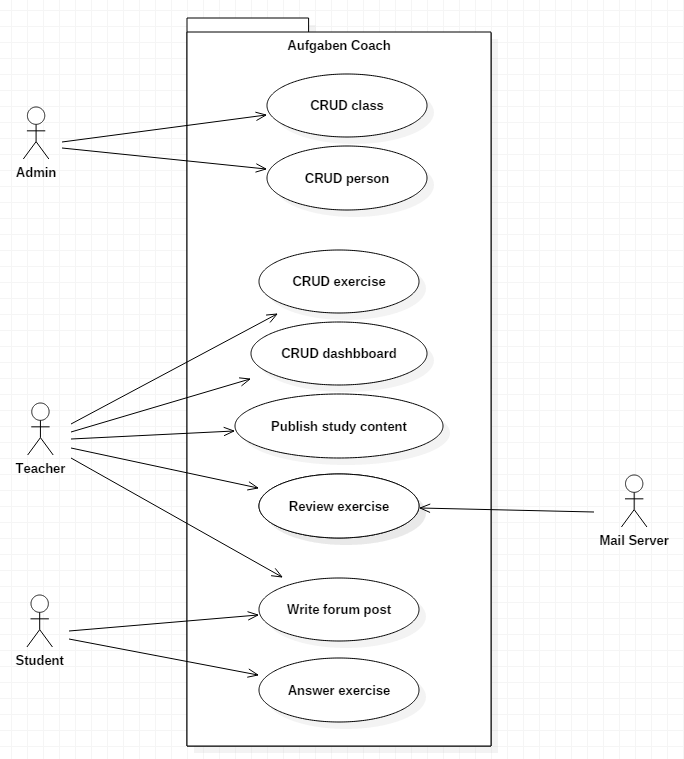
\includegraphics[width=\textwidth, height=\textheight, keepaspectratio]{images/UseCaseDiagramm.png}
	\caption{Use Case Diagramm}
\end{figure}

\end{minipage}


\begin{tabular}{| p{1cm} | p{1.3cm}|}
	\hline
	\textbf{Farbe} & \textbf{Priorität} \\
	\hline	
	grün & hoch \\
	\hline
	orange & tief \\
	\hline
\end{tabular}


\subsubsection{Aktoren}

\begin{table}[H]
	\centering
	\begin{tabu} to 0.9\textwidth {l X}
	\toprule
	Aktor & Beschreibung \\ 
	\midrule
	Administrator & Der Administrator ist für die Verwaltung der Klassen, Lehrer und Schüler zuständig. Er kann Klassen erstellen sowie Lehrpersonen und Schüler diesen Klassen zuweisen. \\
	\midrule
		Lehrer & Der Lehrer verwaltet die ihm zugewiesenen Klassen. Er kann Fächer für seine Klassen freischalten sowie Aufgaben erstellen und diese der Klasse zuweisen. Zusätzlich kann er Statistiken einsehen, die ihn über den aktuellen Wissensstand seiner Klasse informieren. \\
	\midrule
		Schüler & Die Schüler haben Zugriff auf freigeschaltete Lerninhalte und können diese anschauen. Falls Fragen auftreten, können diese im aufgaben-spezifischen Forum gestellt werden. Zusätzlich können Aufgaben gelöst werden. \\
	\bottomrule
	\end{tabu}
	\captionof{table}{Aktoren}
\end{table}


\subsubsection{Beschreibung der Use Cases}
\textbf{UC01: CRUD person}

\noindent Hauptszenario: \\
Ein Administrator kann einen neuen Benutzer erstellen. Dabei kann er zwischen Lehrern und Schülern unterscheiden. Es müssen Angaben wie Vorname, Nachname, Benutzername, E-Mail Adresse und Passwort gemacht werden. Das System erstellt den gewünschten Benutzer, sodass dieser die Applikation ab sofort benutzen kann. \\

\noindent Alternatives Szenario: \\
Ein Administrator löscht eine nicht mehr berechtigte Person aus dem System. \\


\noindent \textbf{UC02: CRUD class}

\noindent Hauptszenario: \\
Ein Administrator erstellt eine neue Klasse. Dabei muss er den Namen der Klasse, wie auch das Eintrittsdatum angeben. Mit Hilfe des Eintrittsdatums kann im späteren Verlauf der Arbeit eine Statistik über mehrere ''Generationen'' von Klassen gemacht werden. \\

\noindent Alternatives Szenario: \\
Ein Administrator löscht eine nicht mehr benötigte Klasse aus dem System. \\


\noindent \textbf{UC03: assigne persons}

\noindent Hauptszenario: \\
Ein Administrator wählt eine bereits erstellte Klasse und weisst dieser eine unbestimmte Anzahl Lehrpersonen zu, sowie auch Schüler, welche noch keiner anderen Klasse zugewiesen wurden. \\

\noindent Alternatives Szenario: \\
Ein Administrator wählt eine bereits erstellte Klasse und entfernt Schüler und/oder Lehrer von dieser. \\


\noindent \textbf{UC04: CRUD exercise}

\noindent Hauptszenario: \\
Ein Lehrer definiert eine neue Aufgabe. Zur Aufgabe erstellt er mehrere Fragen. Zu jeder Frage kann er Hilfestellungen definieren, sowie angeben was die maximale Punktezahl ist. \\

\noindent Alternatives Szenario: \\
Ein Lehrer wählt eine erstellte Aufgabe aus und bearbeitet die Fragen dazu. Das heisst, es können weitere Fragen erstellt, bereits erstellte entfernt, oder aber auch neue Hilfestellungen hinzugefügt werden. \\


\noindent \textbf{UC05: CRUD weekly schedule}

\noindent Hauptszenario: \\
Ein Lehrer erstellt einen Wochenplan. Er erweitert Aufgaben und Quizzes mit einer Deadline und weisst diese einer seiner Klassen zu. \\

\noindent Alternatives Szenario: \\
Ein Lehrer bearbeitet einen bereits erstellten Wochenplan. Die Deadline einer Aufgabe wird um einen oder zwei Tage verschoben. \\


\noindent \textbf{UC06: CRUD quiz}

\noindent Hauptszenario: \\
Ein Lehrer definiert ein Quiz. Dazu erfasst er einige Fragen, die entsprechenden Antwortmöglichkeiten und die Lösungen. \\


\noindent \textbf{UC07: publish study content}

\noindent Hauptszenario: \\
Ein Lehrer schaltet ein neues Fach oder ein neues Thema für eine Klasse frei. \\

\noindent Alternatives Szenario: \\
Ein Lehrer entzieht einer Klasse das Recht ein Fach oder ein Thema zu sehen. \\


\noindent \textbf{UC08: view statistics}

\noindent Hauptszenario: \\
Ein Lehrer wählt eine Klasse und ein ihr zugewiesenes Fach aus. Das System berechnet anhand der von dieser Klasse gelösten Aufgaben eine Statistik und stellt diese dar. Wenn der Lehrer genauere Details sehen will, erstellt das System eine detailiertere Statistik. \\


\noindent \textbf{UC09: use forum}

\noindent Hauptszenario: \\
Ein Schüler sieht das aufgabenspezifische Forum. Findet er nicht die gewünschte Antwort, stellt er selber eine Frage. \\

\noindent Alternatives Szenario: \\
Ein Lehrer sieht, dass ein Schüler eine unbeantwortete Frage hat und beantwortet diese. \\


\noindent \textbf{UC10: send mail}

\noindent Hauptszenario: \\
Das System bemerkt, dass eine von einem Schüler gestellte Frage im Forum über längere Zeit nicht beantwortet wurde und informiert den Lehrer darüber per Mail. \\


\noindent \textbf{UC011: solve exercise}

\noindent Hauptszenario: \\
Ein Schüler löst eine Aufgabe. \\

\noindent Alternatives Szenario: \\
Ein Schüler überarbeitet eine bereits gelöste Aufgabe. \\


\noindent \textbf{UC012: solve quiz}

\noindent Hauptszenario: \\
Ein Schüler löst ein Quiz. \\

\noindent Alternatives Szenario: \\
Ein Schüler überarbeitet ein bereits gelöstes Quiz. \\


\subsection{Nicht Funktionale Anforderungen}
Bei der Erstellung der einzelnen \gls{nfr} wird auf FURPS zurückgegriffen. FURPS ist ein Akronym für Functionality, Usability, Reliability, Performance und Supportability. Dieses Modell wurde im Jahre 1992 von HP entwickelt und dient zur Priorisierung der Software Requirements.\footcite{furps_description}

\begin{table}[h]
	\centering
	\begin{tabu} to 0.9\textwidth {l l X}
	\toprule
	FURPS & Titel & Beschreibung \\ 
	\midrule
	Functionality & User Interface & Das User Interface der Applikation ist über den Webbrowser erreichbar. \\ 
	& Security & Die einzelnen Benutzer können nur auf die für sie freigegebenen Inhalte zugreifen. \\
	& HTTPS & Die Kommunikation zum Webserver soll über HTTS laufen. \\
	\midrule
	Usability & Responsiveness & Für Schüler soll die Applikation sowohl auf Desktop PCs wie auch auf Tablets oder Mobile Phones verfügbar sein. \\
	\midrule
	Reliability & Availability & Die Applikation soll 24/7 verfügbar sein. \\
	 & Fault Tolerance & Die Applikation soll bei unerlaubten Anfragen weiterhin verfügbar sein. \\
	\midrule
	Performance & Response Time & Wechselt der Benutzer zwischen einzelnen Seiten, soll die neue Seite in maximal einer Sekunde geladen worden sein.\\
	\midrule
	Supportability & Maintainability & Die Applikation soll gebaut werden, dass sie auch in Zukunft gewartet und ausgebaut werden kann. \\
	 & Scalability & Die Applikation soll von 300 Benutzern zeitgleich verwendet werden. \\
	\bottomrule
	\end{tabu}
	\captionof{table}{Non Functional Requirements}
\end{table}

%\subsubsection{Functionality}
%\subsubsection*{}
%
%\subsubsection{Qualität}
%Um die Qualität des Codes möglichst hoch zu halten und sicherzustellen, dass alle Teammitglieder immer auf dem aktuellsten Stand sind, werden auf Git Pull-Requests verwendet. Dadurch kann sichergestellt werden, dass ein anderes Teammitglied den geschriebenen Code ebenfalls angesehen und durchdacht hat.
%
%\subsubsection*{Maintainability}
%Die Software könnte unter Umständen in einem Start-Up verwendet werden. Da in Zukunft noch beinahe beliebig viele neue Anforderungen hinzustossen können, soll die Applikation so gebaut werden, dass sie einfach modifiziert werden kann. 
%
%\subsubsection*{Reliability}
%Die Applikation soll robust und reibungslos laufen, auch wenn mehere Schüler zeitgleich mit der Plattform verbunden sind.
%
%\subsubsection*{Scalability}
%Das System soll problemlos von bis zu 300 Benutzern gleichzeitig verwendet werden können. 
%
%\subsubsection*{Usability}
%Bei der Applikation soll es sich um eine Mobile First Applikation handeln. Die Plattform soll sowohl auf Desktop PCs, Tablets und Smartphones bedienbar sein. Der Lehrer- und Administator-spezifische Teil der Applikation ist davon erstmals ausgenommen, da davon ausgegangen wird, dass diese beiden Aktoren hauptsächlich auf Desktop PCs arbeiten. 
%Die Applikation soll ein intuitives User Interface besitzen, damit sich die Benutzer auf Anhieb zurechtfinden. 
%
%\subsubsection*{Security}
%Der Zugriff auf das System ist passwortgeschützt. Benutzer können sich nicht selbstständig registrieren. Nur Administratoren können neue Benutzer erfassen.
%Jede Person sieht nur die Informationen, die für sie selbst von Bedeutung sind. Ein Schüler hat zum Beispiel keinen Zugriff auf die Statistiken anderer Schüler.


\newpage
\section{Architektur}
\subsection{System Übersicht}
Für die Umsetzung der Anwendung gibt es zwei Optionen. Man kann zwischen einer Native App, also einer klassische Client-Server Anwendung, oder eine Web Anwendung, entscheiden. \\

Native Apps haben zwar einige Vorteile. Die Integration mit anderen Anwendungen ist so zum Beispiel einfacher. Zudem wäre die Monetarisierung auch um einiges einfacher, denn eine Native App kann sehr gut im App Store platziert werden. So steigt auch gleich die Bekanntheit der Applikation\footcite{native_app}. \\

Die Entscheidung bei der Entwicklung von Aufgaben-Coach fiel jedoch sehr schnell auf eine Web Anwendung. Viele Schulen haben zwar Apple iPads im Einsatz. Trotzdem kann es Schulen geben, welche mit Android Tablets arbeiten. Mit einer Native App müsste für jedes Betriebssystem ein separates Programm erstellt werden.\\

Hinzu kommt noch die Anforderung der Lehrer. Da diese hauptsächlich auf Notebooks oder Desktop PCs arbeiten, müsste für sie auch eine separate Anwendung entwickelt werden. Mit einer Web Anwendung hat man den Vorteil, nur eine Anwendung entwickeln zu müssen, auf welche alle Benutzer Zugriff haben.\\

Ein weiterer Vorteil von Web Anwendungen ist, dass im vorhinein kein Programm auf dem Device installiert werden muss. Alles, was ein Benutzer braucht, ist ein Internetzugang und ein Tablet. Dies senkt zugleich die Supportkosten der Schule, da so keine Zeit für die Installation oder das Updaten verbraucht wird.

\begin{figure}[H]
\begin{center}
	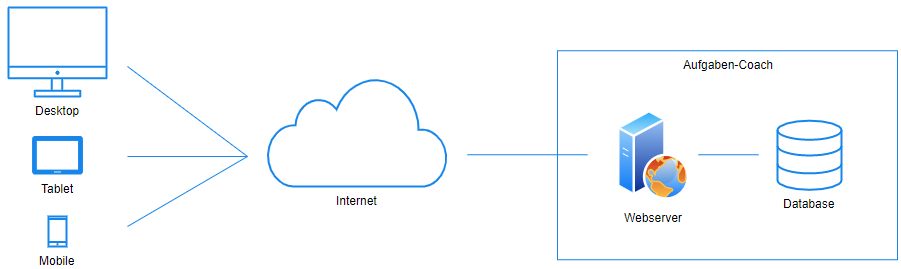
\includegraphics[width=\textwidth, keepaspectratio]{images/system_overview.png}
	\caption{System Overview}
	\label{fig:system_overview}
\end{center}
\end{figure}


\subsection{Domain Model}
In der Abbildung \ref{fig:domain_model_full} ist das vollständige Domain Model abgebildet. Dem Leser soll so ein Überblick über die einzelnen Teilgebiete der Anwendung gegeben werden.

\begin{landscape}

\begin{minipage}{\textwidth}
	\begin{figure}[H]
	\begin{center}
		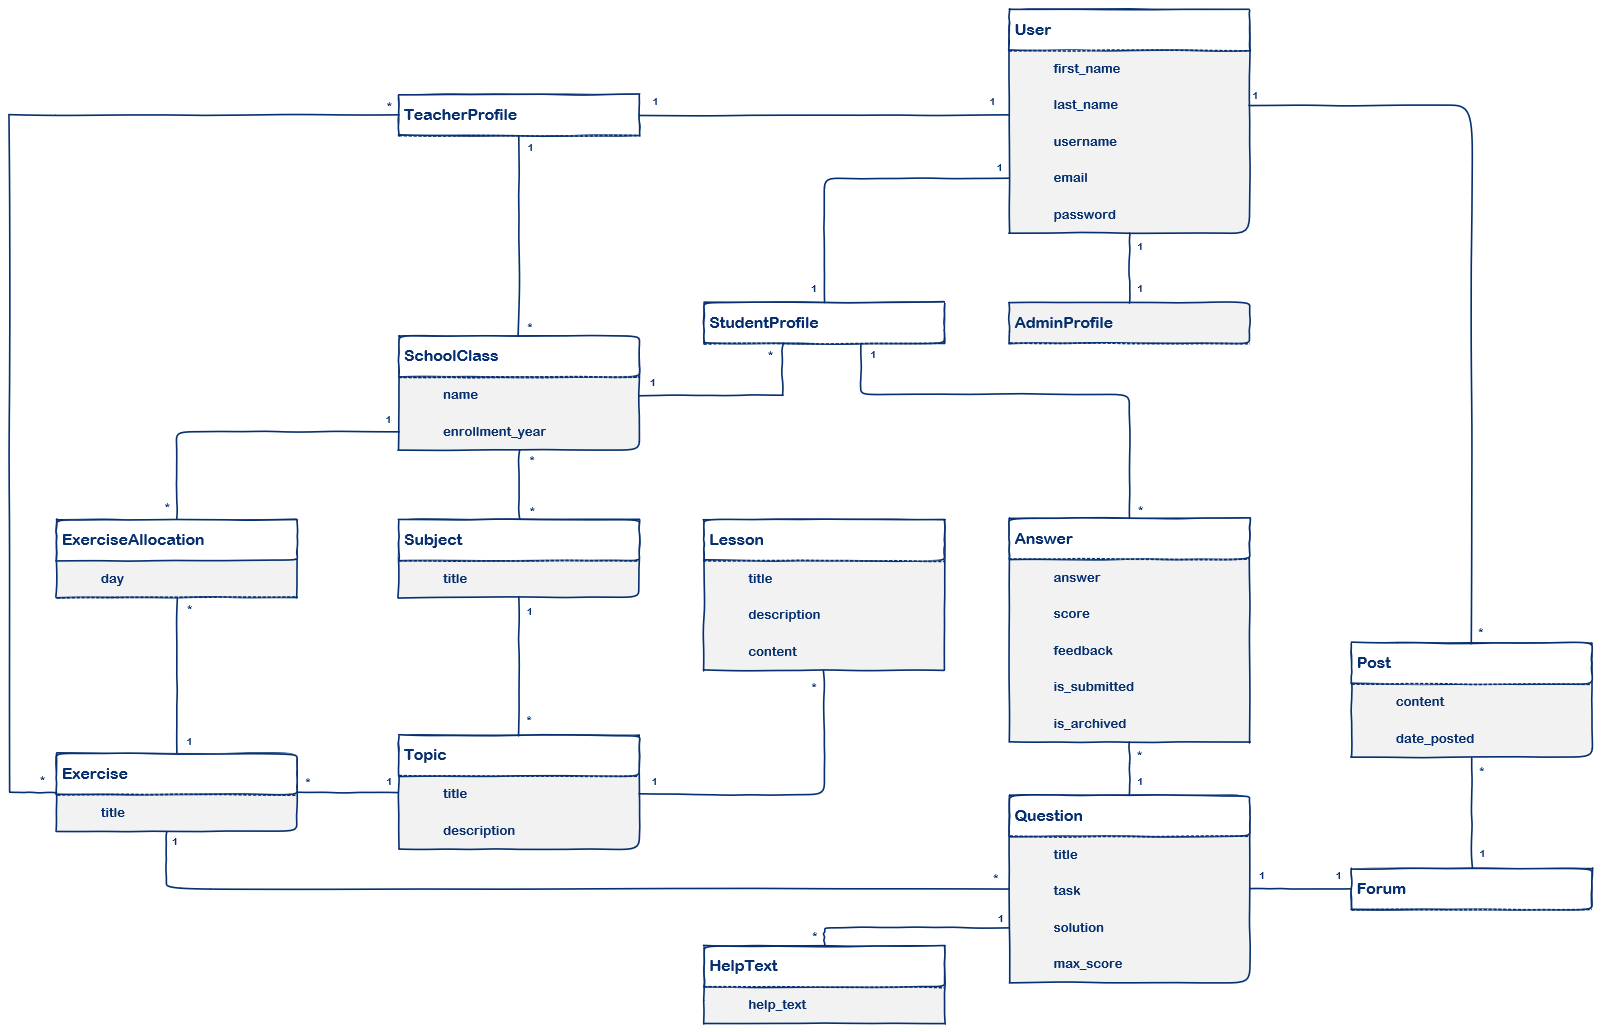
\includegraphics[width=1.4\textwidth, keepaspectratio]{images/domain_model_full.png}
  		\caption{Vollständiges Domain Model}
		\label{fig:domain_model_full}
	\end{center}
	\end{figure}
\end{minipage}

\end{landscape}

%TODO SchoolClass im Domain Model zeigen
\subsubsection*{School}
Ein zentraler Punkt der Anwendung ist die Schule und das User Management. Die User sind einer der drei Rollen Student, Teacher oder Admin zugeteilt. Da jede Rolle unterschiedliche Rechte hat, konnte nicht das Standard User Model von Django selbst verwendet werden. \\
Es stehen drei Möglichkeiten zur Verfügung, wie unterschiedliche User Rollen implementiert werden können.

\begin{enumerate}
	\item Unterscheidung der User anhand eines Boolean Flags
	\item Unterscheidung der User anhand eines Choices Field 
	\item Erstellung eines Profile Models mit einer 1 zu 1 Beziehung zum User Model
\end{enumerate}

Die erste Variante hat den Vorteil, dass ein User mehrere Rollen gleichzeitig haben kann. Im Gegensatz zur ersten Variante kann ein User bei der zweiten Variante nur eine Rolle annehmen. Diese beiden Varianten haben jedoch den Nachteil, dass jeder User die gleichen Daten hat. Möchte man einem Schüler eine Matrikelnummer zuweisen, existiert dieses Feld implizit auch für alle Lehrer und Admins. \\
Um diesem Problem aus dem Weg zu gehen, entschied man sich für die dritte Variante. Pro Rolle existiert ein Profile Model. Möchte man nur einer bestimmten Rolle ein Feld zuweisen, so kann dieses Feld im entsprechenden Profile Model hinzugefügt werden\footcite{django:user_types}. \\

\begin{figure}[H]
	\begin{center}
	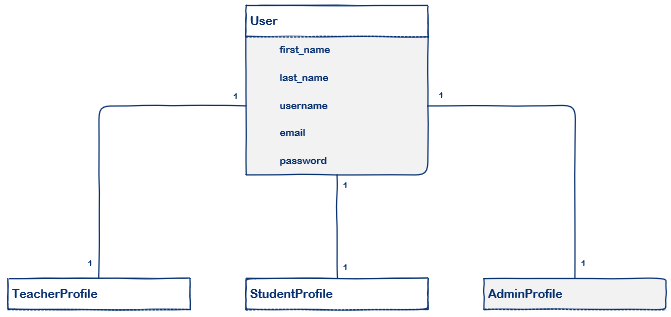
\includegraphics[width=\textwidth, keepaspectratio]{images/domain_model_user.png}
	\caption{Domain Model - User Abschnitt}
	\label{fig:domain_model_user}
	\end{center}
\end{figure}

Der Admin kann als einziger User Typ für sich alleine existieren. Schüler und Lehrer werden Klassen zugewiesen. Ein Lehrer kann gleichzeitig mehreren Klassen zugewiesen sein, ein Schüler kann sich jedoch nur in einer Klasse befinden. Für den aktuellen Stand reicht diese Funktionalität aus. Es gibt jedoch den Use Case, in welchem Schüler aus unterschiedlichen Klassen Fächer zusammen belegen. Dies ist zum Beispiel der Fall, wenn Migrationskinder aus unterschiedlichen Klassen zusammen kommen und gemeinsam ein Deutsch Nachhilfe Fach besuchen. Für diesen Fall kann man dem Student Profile ein Boolean Flag zuweisen. Falls dieses Flag gesetzt ist, hat der Schüler Zugriff auf Nachhilfe Fächer. \\

Wenn dieses Projekt als Startup weiter verfolgt wird, dann würde pro Schule eine neue Instanz der Anwendung deployed werden. So entstehen keine Multi Tenancy Probleme. Möchte man in Zukunft jedoch einen Multi Tenancy Ansatz verfolgen, müsste das Domain Model dementsprechend angepasst werden. Ein möglicher Lösungsansatz wäre, wenn jeder Schule eine eigene Subdomain, wie zum Beispiel schule-gossau.aufgaben-coach.ch, vergeben würde. Anhand der Subdomain können dann die einzelnen User identifiziert werden\footcite{django:multi_tenancy}.

\newpage
%TODO User, StudentProfile und TeacherProfile entfernen
\subsubsection*{Study Content}
Ein zentraler Punkt dieser Anwendung sind die Schulfächer. Pro Subject gibt es mehrere Topics. Topics wiederum können mehrere Lessons haben. \\ 

\begin{figure}[H]
\begin{center}
	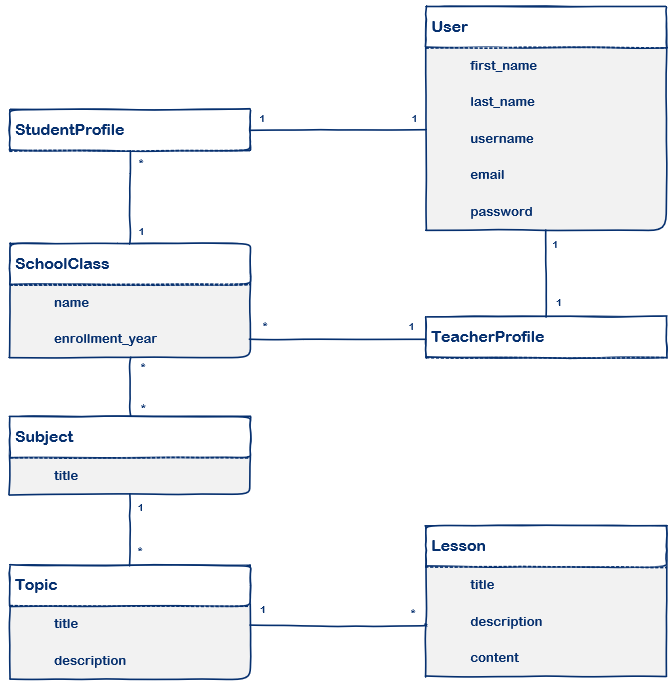
\includegraphics[width=\textwidth, keepaspectratio]{images/domain_model_study_content.png}
	\caption{Domain Model - Schulfächer}
	\label{fig:domain_model_study_content}
\end{center}
\end{figure}


Ein Subject kann einer Klasse zugewiesen werden. Erst dann hat die Klasse Zugriff auf Topics und Lessons. Im Moment ist es nicht möglich, einzelne Topics oder Lessons freizuschalten. Möchte man diese Funktionalität in Zukunft jedoch haben, muss eine neue Zwischentabelle in der Datenbank erstellt werden.

\newpage
\subsubsection*{Exercise}
Das Herzstück der Anwendung sind die Exercises. Lehrer können Übungen erstellen, welche aus mehreren Teilaufgaben bestehen, welche wiederm mehrere Hilfestellungen haben. 

\begin{figure}[H]
\begin{center}
	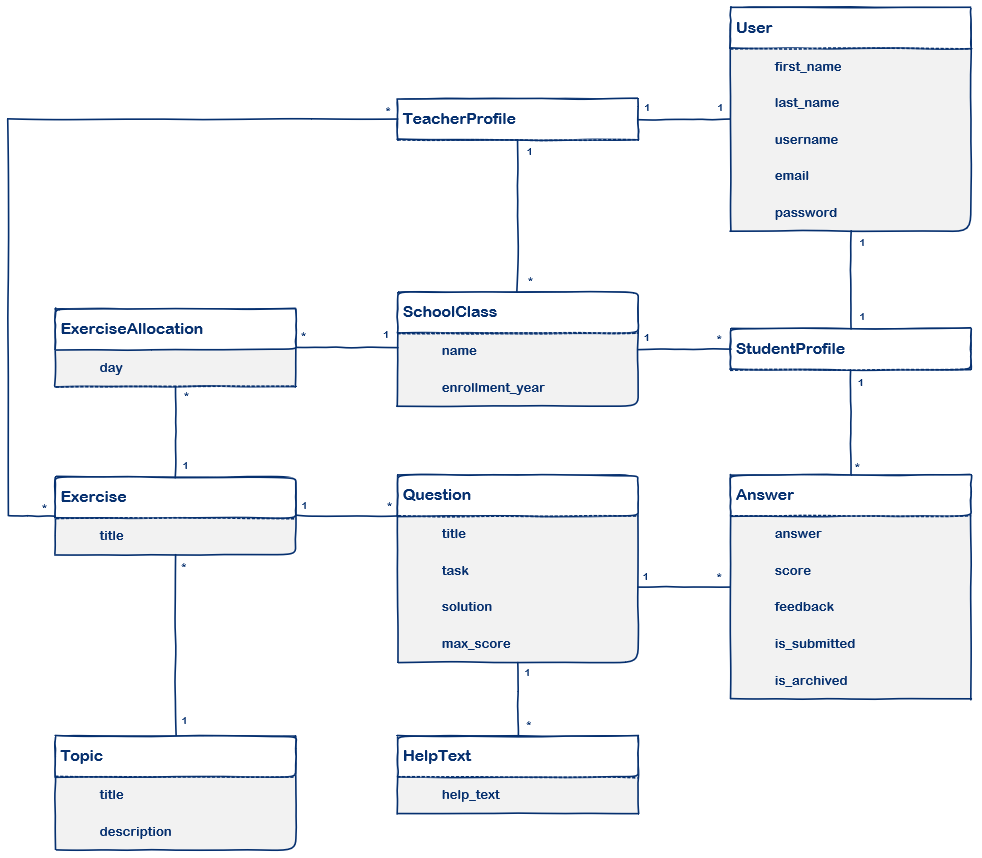
\includegraphics[width=\textwidth, keepaspectratio]{images/domain_model_exercise.png}
	\caption{Domain Model - Aufgaben}
	\label{fig:domain_model_exercise}
\end{center}
\end{figure}

Die Tabelle Answer dient zur Speicherung der Antworten von Schülern. Die beiden Felder ''is\_submitted'' und ''is\_archived'' sind für den Status der Aufgaben. Ist eine Aufgabe submitted, also abgegeben, kann sie nicht weiter vom Schüler bearbeitet werden. Erst wenn Aufgaben abgegeben sind, können sie vom Lehrer angeschaut werden. \\ 
Wurden die Aufgaben vom Lehrer korrigiert, bekommen sie den Status ''is\_archived''.

\newpage
\subsubsection*{Forum}
Für jede Frage in einer Übung gibt es ein Forum. Die Schüler haben einen Ort, in welchem Fragen gestellt werden können. Da es für jede Frage ein Forum gibt, werden die Schüler auch nicht von anderen Forumsbeiträgen abgelenkt.
\begin{figure}[H]
\begin{center}
	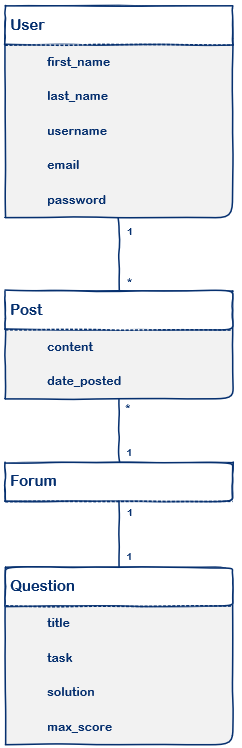
\includegraphics[width=0.3\textwidth, keepaspectratio]{images/domain_model_forum.png}
	\caption{Domain Model - Forum}
	\label{fig:domain_model_forum}
\end{center}
\end{figure}


\subsection{Tools und Frameworks}
Bei der Wahl von Technologien, Tools und Frameworks achtete man besonders darauf, dass die entsprechenden Tools auch in der Zukunft noch supported werden. Dazu wurde geschaut, ob und wie gross die Community hinter einzelnen Tools ist und wie gut die Tools dokumentiert sind.

\subsubsection*{Programmiersprache}
Für das Web Development gibt es mehrere Programmiersprachen, die zur Auswahl standen. Die Wohl bekanntesten darunter sind:

%https://en.wikipedia.org/wiki/Web_framework

\begin{itemize}
	\item Python (Django / Flask)
	\item C\# (ASP.NET Core)
	\item Java (Spring)
	\item JavaScript (Express.js / Node.js / Sails.js)
	\item PHP (CakePHP / CodeIgniter / Laravel)
	\item Perl (Catalyst / Mojolicious)
	\item Ruby (Ruby on Rails)
\end{itemize}

%TODO Satzstellung anschauen

Gemäss Developer Survey Results\footcite{developer_survey_results} von Stack Overflow ist Python (41.7\%) etwas beliebter als Java (41.1\%). Nur JavaScript (67.8\%) ist noch bekannter. In den letzten Jahren ist die Bekanntheit von Python noch weiter gestiegen. \\

Die Wahl der Programmiersprache fiel schnell auf Python, da bereits etwas KnowHow vorhanden ist. Man geht aber davon aus, dass Python in Zukunft noch an Beliebtheit steigt und man weiterhin damit arbeiten kann.


\subsubsection*{Web Framework}
Mit Python hat man die Auswahl von verschiedenen Web Frameworks. Gemäss einer Umfrage von JetBrains\footcite{python_survey_results} wird die Frage ''What web frameworks / libraries do you use in addition to Python?'' mit dem Kommentar ''Django and Flask continue to be by far the most popular Python web frameworks.'' zusammengefasst. \\
Laut der oben genannten Umfrage verwenden 43\% der Entwickler  Django als Web Framework. Flask folgt dicht darauf mit 41\%. Das nächst bekannteste Framework ist Tornado mit nur noch 6\%. \\
Bei der Evaluation konzentrierte man sich deshalb hauptsächlich auf Django und Flask. Mit bekannteren Frameworks hat man den Vorteil, dass es einfacher ist, Hilfe und gute Dokumentationen zu finden. Mit weit verbreiteten Technologien kann man auch davon ausgehen, dass diese noch längere Zeit bestehen bleiben.  \\ 

%TODO zitat einbauen
Flask\footcite{flask:foreword} beschreibt sich selber mit den Worten:

\begin{displayquote}
Flask is a lightweight WSGI web application framework. It is designed to make getting started quick and easy, with the ability to scale up to complex applications. It began as a simple wrapper around Werkzeug and Jinja and has become one of the most popular Python web application frameworks. \\
Flask offers suggestions, but doesn't enforce any dependencies or project layout. It is up to the developer to choose the tools and libraries they want to use. There are many extensions provided by the community that make adding new functionality easy.
\end{displayquote}

Bei der Studienarbeit verwendete man bereits Flask zum Erstellen einer Web Anwendung. Flask ist sicherlich ein gutes Framework, sonst würde es nicht von 41\% der Entwickler genutzt. Der grosse Vorteil von Flask ist, dass man als Entwickler relativ frei ist, wie man etwas umsetzen möchte. So kommt Flask standardmässig ohne Database Abstraction Layer, Form Validation oder anderen Tools, da bereits Libraries existieren, welche dies erledigen\footcite{flask:design}. Gerade am Anfang kann dies jedoch eher Verwirrung stiften, weil für das selbe Problem mehrere Lösungsmöglichkeiten bereit stehen. \\

Django verfolgt dagegen eher den Ansatz, bereits unterschiedliche Funktionalitäten mitzuliefern, was den Entwicklern Arbeit abnehmen soll. So ist zum Beispiel bereits ein OR-Mapper oder ein Admin Interface integriert\footcite{django:overview}. 
Django hat aber auch ein paar Nachteile. Da einige Entscheidungen bereits vom Framework selber getroffen wurden, ist man als Entwickler nicht mehr ganz so flexibel. Zudem ist Django sehr monolithisch. Bei bestimmten Aufgaben ist vorgegeben, wie diese in Django umgesetzt werden müssen. Hält man sich nicht an den ''Django Way'', kann unter Umständen die gesamte Anwendung nicht deployed werden\footcite{django:advantages_disadvantages}.

In der Studienarbeit konnte man zwar bereits Erfahrung mit Flask sammeln, dennoch entschied man sich für Django. Besonders dass das Django als ''Fully Loaded Framework'' und mit einem integrierten Admin Interface daher kommt, wurde als sehr positiv erachtet.


\subsubsection*{Datenbank}
Um ein Datenbanksystem kommt diese Anwendung nicht herum. Folgende Überlegungen wurden sich bei der Evaluation für eine geeignete Datenbank gemacht:

\begin{itemize}
	\item Die Datenbank muss skalierbar sein, so dass sie auch eine grosse Anzahl Benutzer unterstützt.
	\item Da ein Grossteil der Benutzer mit Mobile Devices auf die Anwendung zugreift, soll bei Anfragen möglichst wenig Overhead geliefert werden.
	\item Die Schreib- und Lese-Operationen sind wichtig, jedoch nicht kritisch. 
\end{itemize}

Aufgrund der ohnehin schon verkürzten Projektlaufzeit entschied man sich, auf die Evaluation eines Datenbanksystems zu verzichten. Während den Modulen Datenbanksysteme 1 \& 2 konnte bereits sehr viel Erfahrungen mit Postgres gesammelt werden. Laut Deployment Statistics\footcite{deploymentstatistics} von Django Sites verwenden 47.7\% aller deployten Sites MySQL als Datenbank. Postgres folgt mit 40.7\%. Das nächst grössere Datenbanksystem ist sqlite mit nur noch 7.6\%.
MySQL wird zwar etwas öfters verwendet. Aus Erfahrung weiss man aber, dass die Funktionen von Postgres die Bedürfnisse dieser Anwendung voll und ganz abdecken, weshalb man Postgres als Datenbanksystem festlegte. \\

Sollte man in Zukunft jedoch ein anderes Datenbanksystem bevorzugen, kann die Migration mit dem Django Management Tool durchgeführt werden \footcite{dbmigration}. 

\subsubsection*{Python Libraries}
Libraries beschreiben


\subsection{Deployment}
Zusätzlich zur System Overview in Abbildung \ref{fig:system_overview}, wird hier das Deployment Diagramm gezeigt. Dieses soll die einzelnen Komponenten aufzeigen.

\begin{figure}[H]
\begin{center}
	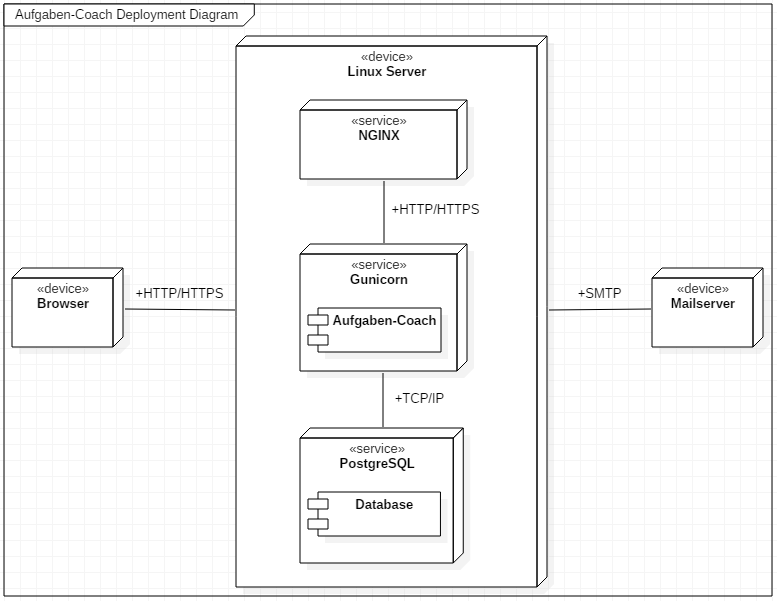
\includegraphics[width=\textwidth, keepaspectratio]{images/deployment_diagram.png}
	\caption{Deployment Diagramm}
	\label{fig:deployment_diagram}
\end{center}
\end{figure}

\subsubsection*{Web Server}
Bei der Evaluation eines Web Servers beschränkte man sich auf NGINX und Apache. Wie man auf einer Statistik von w3techs\footcite{webserver_usage} entnehmen kann, wird in 42\% der Web Server Apache eingesetzt. NGINX kommt mit 31.3\% etwas weniger zum Einsatz. \\

Apache kommt öfters zum Einsatz und ist flexibler als NGINX\footcite{webserver_comparison}. Dennoch entschied man sich für NGINX. Bei dieser Entscheidung achtete man hauptsächlich auf die Performance der beiden Web Server, bei welcher NGINX in den Kategorien ''Requests per second'', ''Time per request'' und ''Transfer rate'' durchschnittlich besser abschnitt\footcite{webserver_performance}.

\subsection*{Web Server Gateway Interface}
Während der Entwicklungsphase wurde der Development Server, welcher direkt mit dem Django Framework mitgeliefert wird, verwendet. In der produktiven Umgebung reicht dies jedoch nicht mehr aus, weshalb ein \gls{wsgi} eingesetzt wird. Dieser beschreibt, wie der Web Server mit einer Web Anwendung kommuniziert. Anfragen an den Web Server werden zur Web Anwendung geleitet. Sobald der Request bearbeitet wurde, wird die Response an den Web Server zurück geschickt\footcite{wsgi_description}.


%\subsection{Analyse (Business Model)}
\subsubsection{Domain Model}
In der nachfolgenden Abbildung ist das vollständige Domain Model Model abgebildet. Um dem Leser ein klares Bild zu verschaffen, wurde dieses in die einzelnen Teilbereiche aufgeteilt.

\subsubsection*{Schule}
Ein zentraler Punkt der Anwendung ist die Schule an sich und das User Management. Wenn dieses Projekt als Startup weiter verfolgt wird, dann würde pro Schule eine neue Instanz der Anwendung deployed. So entstehen auch keine Probleme wegen dem Multi Tenancy. Würde man in Zukunft jedoch doch lieber einen Multi Tenancy Ansatz verfolgen, müsste das Domain Model dementsprechend angepasst werden. Ein möglicher Lösungsansatz wäre, wenn man jeder Schule eine eigene Subdomain, wie zum Beispiel schule-gossau.aufgaben-coach.ch, vergeben würde. Anhand der Subdomain können dann die einzelnen User identifiziert werden.
% https://books.agiliq.com/projects/django-multi-tenant/en/latest/shared-database-shared-schema.html
Jeder User ist einer von drei Rollen Student, Teacher oder Admin zugeteilt. Da jede Rolle unterschiedliche Rechte hat, konnte nicht das Standard User Model von Django selber verwendet werden. Nach der Recherche standen drei Möglichkeiten zur Verfügung.

\begin{enumerate}
	\item Unterscheidung der User anhand eines Boolean Flags
	\item Unterscheidung der User anhand eines Choices Field 
	\item Erstellung eines Profile Models mit einer 1 zu 1 Beziehung zum User Model
\end{enumerate}

Die erste Variante hat den Vorteil, dass ein User mehrere Rollen gleichzeitig haben kann. Im Gegensatz zur ersten Variante kann ein User bei der zweiten Variante nur eine Rolle annehmen kann. Diese beiden Varianten haben jedoch den Nachteil, dass jeder User die gleichen Daten hat. Möchte man einem Schüler eine Matrikelnummer zuweisen, existiert dieses Feld implizit auch für alle Lehrer und Admins. \\
Um diesem Problem aus dem Weg zu gehen, entschied man sich für die dritte Variante. Pro Rolle existiert ein Profile Model. Möchte man Felder nur einer bestimmten Rolle zuweisen, so kann dieses Feld im entsprechenden Profile Model hinzugefügt werden. \\
Der Admin kann als einziger User Typ für sich alleine existieren. Schüler und Lehrer werden Klassen zugewiesen. Ein Lehrer kann gleichzeitig mehreren Klassen zugewiesen sein, ein Schüler kann sich jedoch nur in einer Klasse befinden. Für den aktuellen Stand reicht diese Funktionalität aus. Es gibt jedoch den Use Case, in welchem Schüler aus unterschiedlichen Klassen Fächer zusammen belegen. Dies ist zum Beispiel der Fall, wenn Migrationskinder aus unterschiedlichen Klassen zusammen kommen und gemeinsam ein Deutsch Nachhilfe Fach besuchen. Für diesen Fall kann man dem Student Profile ein Boolean Flag zuweisen. Falls dieses Flag gesetzt ist, hat der Schüler Zugriff auf Nachhilfe Fächer.

% https://simpleisbetterthancomplex.com/tutorial/2018/01/18/how-to-implement-multiple-user-types-with-django.html
\subsection{Design}
\subsubsection{Architektur und Abhängigkeiten}
Bei der Wahl von Technologien, Tools und Frameworks achtete man besonders darauf, 
%TODO
\subsubsection*{Applikations Architektur}
Für die Umsetzung der Anwendung hatte man zwei Optionen. Entweder man entwickelt eine Native App, also eine klassische Client-Server Anwendung, oder eine Web Anwendung. \\

Native Apps haben zwar einige Vorteile. Die Integration mit anderen Anwendungen wäre so zum Beispiel einfacher. Zudem wäre die Monetarisierung 	auch um einiges einfacher, denn eine Native App könnte man sehr gut im App Store platzieren. So würde auch gleich die Bekanntheit der Applikation steigen. \\

Die Entscheidung bei der Entwicklung von Aufgaben-Coaching viel jedoch sehr schnell auf eine Web Anwendung. Viele Schulen haben zwar Apple iPads im Einsatz. Trotzdem kann es Schulen geben, welche mit Android Devices arbeiten. Da die Anwendung aber über den Browser läuft, muss nur eine Anwendung entwickelt werden. Bei einer Native App müsste man für Apple und Android je eine Anwendung entwickeln. Für grosse Firmen ist dies kein Problem, aber möchte man die Idee als Startup weiter verfolgen, hätte man weder die Zeit noch das Kapital um gleich zwei Apps zu entwickeln. \\
Zudem kann man mit Web Anwendungen die Supportkosten relativ tief halten, was auf Schulen vielleicht noch ein bisschen attraktiver wirkt. Die Anwendung kann direkt im Browser aufgerufen werden und es muss nichts im vorhinein auf dem Device installiert werden.

% http://www.differencebetween.net/technology/software-technology/difference-between-client-server-application-and-web-application/	
% https://www.adjust.com/blog/native-app-vs-progressive-web-app/

\subsubsection*{Programmiersprache}
Für das Web Development gibt es mehrere Programmiersprachen, die zur Auswahl standen. Die Wohl bekanntesten darunter sind:

%https://en.wikipedia.org/wiki/Web_framework

\begin{itemize}
	\item Python (Django / Flask)
	\item C\# (ASP.NET Core)
	\item Java (Spring)
	\item JavaScript (Express.js / Node.js / Sails.js)
	\item PHP (CakePHP / CodeIgniter / Laravel)
	\item Perl (Catalyst / Mojolicious)
	\item Ruby (Ruby on Rails)
\end{itemize}

%TODO Satzstellung anschauen

Die Wahl fiel schnell auf Python, da wir beide am meisten Knowhow über Python verfügen. \\
Gemäss Developer Survey Results von Stack Overflow ist Python (41.7\%) etwas bekannter als Java (41.1\%). Nur JavaScript (67.8\%) ist noch bekannter. In den letzten Jahren ist die Bekanntheit von Python auch noch weiter gestiegen. Man geht also davon aus, dass man auch in Zukunft noch mit Python arbeiten kann.

% https://insights.stackoverflow.com/survey/2019#technology

\subsubsection*{Web Framework}
Bei Python selber steht man vor der Auswahl von verschiedenen Web Frameworks. Gemäss einer Umfrage von JetBrains über Python wird die Frage ''What web frameworks / libraries do you use in addition to Python?'' mit dem Kommentar ''Django and Flask continue to be by far the most popular Python web frameworks.'' zusammen gefasst. \\
Laut der oben genannten Umfrage verwenden 43\% der Entwickler  Django als Web Framework. Flask folgt dicht darauf mit 41\%. Das nächst bekannteste Framework ist Tornado mit nur 6\%. \\
Bei der Evaluation konzentrierte man sich deshalb hauptsächlich auf Django und Flask. Mit bekannteren Frameworks hat man den Vorteil, dass es einfacher ist, Hilfe und gute Dokumentationen zu finden. Mit weit verbreiteten Technologien kann man auch davon ausgehen, dass diese noch längere Zeit bestehen bleiben.  \\ 

Flask beschreibt sich selber mit den Worten:

''Flask is a lightweight WSGI web application framework. It is designed to make getting started quick and easy, with the ability to scale up to complex applications. It began as a simple wrapper around Werkzeug and Jinja and has become one of the most popular Python web application frameworks. \\
Flask offers suggestions, but doesn't enforce any dependencies or project layout. It is up to the developer to choose the tools and libraries they want to use. There are many extensions provided by the community that make adding new functionality easy.''

Bei der Studienarbeit verwendete man bereits Flask zum Erstellen einer Webanwendung. Flask ist sicherlich ein gutes Framework, sonst würde es nicht von 41\% der Entwickler genutzt. Der grosse Vorteil von Flask ist, dass man als Entwickler relativ frei ist, wie man etwas umsetzen möchte. So kommt Flask standardmässig ohne Database Abstraction Layer, Form Validation oder anderen Tools, da bereits Libraries existieren, welche dies erledigen. Gerade am Anfang kann dies jedoch eher Verwirrung stiften, weil für das selbe Problem mehrere Lösungen bereit stehen. \\
% https://flask.palletsprojects.com/en/1.1.x/foreword/

Django verfolgt dagegen eher den Ansatz, bereits unterschiedliche Funktionalitäten mitzuliefern, was den Entwicklern Arbeit abnehmen soll. So ist zum Beispiel bereits ein OR-Mapper oder ein Admin Interface integriert. 
Django kommt aber auch mit einigen Nachteilen. Da einige Entscheidungen bereits vom Framework selber getroffen wurden, ist man als Entwickler nicht mehr ganz so flexibel. Zudem ist Django sehr monolithisch. Bei bestimmten Aufgaben ist vorgegeben, wie diese in Django umgesetzt werden müssen. Hält man sich nicht an den ''Django Way'', kann unter Umständen die gesamte Anwendung nicht deployed werden.

% https://docs.djangoproject.com/en/3.0/intro/overview/
% https://data-flair.training/blogs/django-advantages-and-disadvantages/

In der Studienarbeit konnte man zwar bereits Erfahrung mit Flask sammeln, dennoch entschied man sich für Django. Besonders das Django als ''Fully Loaded Framework'' und mit einem integrierten Admin Interface daher kommt, wurde als sehr positiv erachtet.


\subsubsection*{Datenbank}
Um ein Datenbanksystem \autocite{test123} kommt \footcite{test123} diese Anwendung nicht herum. Folgende Überlegungen wurden sich bei der Evaluation für eine geeignete Datenbank gemacht:

\begin{itemize}
	\item Die Datenbank muss skalierbar sein, so dass sie auch eine grosse Anzahl Benutzer unterstützt.
	\item Da ein Grossteil der Benutzer mit Mobile Devices auf die Anwendung zugreift, soll bei Anfragen möglichst wenig Overhead geliefert werden.
	\item Die Schreib- und Lese-Operationen sind wichtig, jedoch nicht kritisch. 
\end{itemize}

% https://www.quora.com/How-can-we-evaluate-how-good-a-database-is-What-are-the-criteria-for-database-evaluation-Are-there-any-papers-on-the-subject



\subsubsection*{Python Libraries}

\subsubsection{UI Design}
Bevor man mit der Entwicklung des Frontends beginnen konnte, musste geplant werden, wie das User Interface genau aussehen soll. Mit Hilfe der Use Cases konnte ein erster Entwurf erstellt werden. 

\subsection{Mockup}

\newpage



\subsection{Effektive Webseite}

\newpage
\section{Implementation und Tests}
\subsection{Django Architektur}
Bei der Implementation der Anwendung befolgte man die vom Django Framework vorgegebene Architektur. Für die einzelnen Apps entschied man sich jedoch dafür, diese in einem separaten ''apps'' Verzeichnis zu speichern, damit das Home-Verzeichnis übersichtlicher ist.\\

Django ist nach dem \gls{mtv} Pattern aufgebaut, was eine leichte Abänderung des \gls{mvc} Pattern ist. Beim \gls{mvc} Pattern dient das Model als Vermittler zwischen dem Website Interface und der Datenbank. Die View ist das eigentliche User Interface und enthält zum Beispiel das HTML oder CSS der Website. Der Controller ist die Hauptkomponente in diesem Pattern. Er nimmt die korrekte View aus der User Anfrage und weist es dem Model zu\footcite{django_mvc}. \\

Django basiert aber auf dem \gls{mtv} Pattern. Wird im Browser eine \gls{url} aufgerufen, entscheidet Django anhand der \gls{url} Patterns, an welche View die Anfrage gesendet wird. Diese View generiert dann schlussendlich die Webseite mit Hilfe des Templates. \\

%Das Model enthält immer noch die logische Datenstruktur. Die View hat Zugriff auf das Model und kann so Daten speichern, updaten oder löschen. Erhält die View Daten vom Model, kann diese mit dem Template dargestellt werden. Das Template dient lediglich zur Darstellung der einzelnen Webseiten\footcite{django_mtv}.

\begin{figure}[H]
	\begin{center}	
		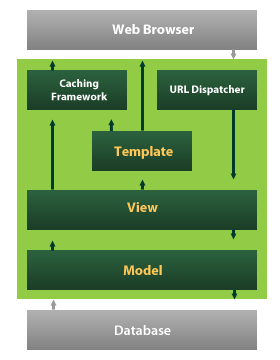
\includegraphics[width=0.5\textwidth, keepaspectratio]{images/django_mtv.png}
		\caption{Django Architektur Diagramm\footcite{django_architektur_image}}
			\label{django_architecture}
	\end{center}
\end{figure}

\subsubsection*{Model}
In den Models wird das Datenbank Model mit den benötigten Feldern erstellt\footcite{django_models}. Django stellt auch gleich einen \gls{orm} bereit, mit welchem die Tabellen in der Datenbank erstellt werden kann. Dies bietet gleich meherere Vorteile. Zum einen nimmt dieser \gls{orm} viel Arbeit ab, da man eigentlich keine Queries schreiben muss. Zum anderen ist es sehr hilfreich, wenn man Migrationen an der Datenstruktur durchführen möchte. Der \gls{orm} erkennt, was an der Datenbank geändert wurde und wie die Daten migriert werden müssen\footcite{django_manage}. Als Entwickler kann man so auch ohne viel Datenbank Kenntnisse einfach Migrationen durchführen.

\subsubsection*{Templates}
Mit Templates können dynamische HTML Seiten generiert werden. Die Templates bestehen aus dem statischen HTML Code, welcher mit dynamischen Inhalten gefüllt werden kann.  Dazu verwendet Django die \gls{dtl}\footcite{django_templates}.

\subsubsection*{Views}
Eine View ist nichts anderes als eine Python Funktion, welche einen Request entgegen und eine Response zurück schicken. Die Response kann alles enthalten, von einfachem \gls{html} bis zu 404 Seiten oder Redirects. Die View an sich enthält die Logik, welche nötig ist, um den Request entgegennehmen zu können oder die Response zu senden\footcite{django_views}.

\subsubsection*{Middlewares}
Hinzu kommen jedoch noch die Django Middlewares, welche Requests und Responses anpassen können. Jede dieser Middlewares ist für bestimmte Funktionen verantwortlich. Die ''AuthenticationMiddleware'' wird zum Beispiel verwendet, um die Benutzer einer Session zuordnen zu können. Es werden auch mehrere Security Middlewares angeboten, welche praktisch ''out-of-the-box'' verwendet werden können. Diese können die Sicherheit der Webseite, zum Beispiel die Integration von \gls{hsts} oder \gls{xss} Schutz, erhöhen\footcite{django_middlewares}.\\


%TODO vielleicht
%\subsection{Apps}
%Bei Django werden unabhängige Funktionalitäten in unterschiedliche Apps aufgeteilt. Eine App in Django ist eigentlich nichts anderes als ein Python Package, welches eine Reihe von Features zur Verfügung stellt\footcite{django:apps}. Das Ziel dabei ist es, den Code auf die verschiedenen Apps aufzuteilen, so dass diese unabhängig voneinander wiederverwendet werden können.  \\
%In der Tabelle \ref{table:django_apps} sind die einzelnen Apps aufgelistet, welche für Aufgaben-Coaching erstellt wurden.
%
%\begin{table}[h]
%	\centering
%	\begin{tabu} to 0.9\textwidth {l X}
%	\toprule
%	App & Beschreibung \\ 
%	\midrule	
%	user & In der Users App befindet sich die gesamte Logik zum erstellen und verwalten der User. \\
%	\midrule
%		school\_admin & Die school\_admin App ist für die Erstellung von Klassen sowie der Zuweisung von Schülern und Lehrern in Klassen zuständig. \\
%	\midrule
%	school\_teacher & In dieser App können Lehrer die Fächer für ihre Klasse freischalten und Aufgaben dem Wochenplan hinzufügen. \\
%	\midrule
%		exercise & Die exercise App stellt um Aufgaben zu erstellen zur Verfügung. Zudem können gelöste Aufgaben von einem Lehrer bewertet werden. \\
%	\midrule 
%	study\_content & Diese App beinhaltet die Logik zum bereitstellen von Lerninhalten \\
%	\midrule	
%	forum & In der forum App wird die komplette Logik für das Forum implementiert. \\
%	\bottomrule
%	\end{tabu}
%	\captionof{table}{Apps Beschreibung}
%	\label{table:django_apps}
%\end{table}


\subsection{Testing}
Es gibt mehrere Arten von Tests, welche durchgeführt wurden, um die Qulität dieser Arbeit zu gewährleisten.

\subsubsection{Unit Tests}
Anhand der Unittests werden die erstellten Models getestet. Mit diesen Tests wird sichergestellt, dass die Models korrekt funktionieren. Es kann zum Beispiel getestet werden, ob die Objekte als String abgespeichert werden oder ob duplizierte Objekte abgelegt werden können. Wenn in der Datenbank bereits ein Subject mit dem Titel ''Mathematik'' existiert, darf kein weiteres Subject mit dem selben Namen erstellt werden können.


\subsubsection{Integration Tests}
Mit Integration Tests kann getestet werden, ob die Applikation korrekt auf eingehende Requests reagiert. Diese Anwendung wird von mehreren Benutzern mit unterschiedlichen Rechten verwendet. Beim Erstellen der Tests wurde besonders viel Wert darauf gelegt, dass geprüft wird, dass jeder Benutzer nur Zugriff auf die erlaubten Webseiten hat. Aus Erfahrung weiss man, dass Schüler sehr experimentierfreudig sind und sicherlich versuchen werden, die \gls{url} des Browsers anzupassen. Es darf jedoch nicht vorkommen, dass ein Schüler Zugriff auf Statistiken hat oder die Punktezahl von Aufgaben anpassen kann.


\subsubsection{Manuelle Tests}
Manuelle Tests wurden da eingesetzt, wo es sehr schwierig und Zeitaufwändig gewesen wäre, Tests zu schreiben. Vor jedem Merge in den Master wurde geprüft, ob diese Funktionen noch funktionieren. Ein Beispiel für den Fall von manuellen Tests ist zum Beispiel, ob das Filtering und Pagination noch funktioniert. Zu Beginn hatte man da das Problem, dass das Filtern zwar funktionierte, aber das Pagination basierte auf dem gesamten Queryset. Die Anzahl der Seiten änderte sich also nicht, auch wenn der Filter kein einziges Element gefunden hat. Ein weiterer Fall für manuelle Tests sind die Drag\&Drop Seiten. Bei diesen wurde geprüft, ob man das Item einem Feld zuweisen kann und ob es anschliessend richtig in der Datenbank gespeichert wird. \\


\subsubsection{Usability Tests}
Nachdem man die Mockups erstellt hat, konnten damit die Usability Tests durchgeführt werden. Ziel dieser Tests ist es, zu prüfen, ob Benutzer das Design der Webseite verstehen und wissen, wo man was machen kann. \\

%TODO balsamiq i de mockups beschriibe, ned bim teste
Jeder der 3 Probanden hat die Tests für alle drei Benutzerrollen durchgeführt. Bei jeder Durchführung sollten sie jedoch eine andere Rolle und andere Aufgaben übernehmen. So konnte verhindert werden, dass die Tests verfälscht werden. Auch wenn einer der Probanden die Webseite gesehen hat, musste er jedes Mal andere Aufgaben lösen. Zudem löste jeder Proband die Tests in einer anderen Reihenfolge. Somit hat man zumindest für den ersten Test eine Person, welcher die Webseite noch nie gesehen hat. \\
In der Tabelle \ref{usability_test_rollen} ist ein Beispiel, wie die Durchführung der Tests gemacht wurde.

%Die Usability Tests wurden mit den in der Planung erstellen Mockups durchgeführt. Die Mockups wurden mit der  Balsamiq\footcite{balsamiq_mockups} erstellt. Bereits während des Engineering Projekts und der Studienarbeit konnten damit Erfahrungen gesammelt werden. Zudem ermöglicht es Balsamiq relativ leicht, schöne interaktive Mockups zu erstellen. Durch interaktive Mockups kann die Qualität der Usability Tests verbessert werden, da es sich für die Probanden echter anfühlt und sie dadurch mit grösserer Wahrscheinlichkeit so reagieren, wie sie es dann auf der effektiven Webseite tun werden \footcite{interactive_mockups}. \\


\begin{table}[h]
	\centering
	\begin{tabu} to 0.9\textwidth {l X X X}
	\toprule
		Proband & Durchführung 1 & Durchführung 2 & Durchführung 3 \\ 
	\midrule
		Proband 1 & Schüler & Lehrer & Administrator \\
		Proband 2 & Lehrer & Administrator & Schüler \\
		Proband 3 & Administrator & Lehrer & Schüler \\
	\bottomrule
	\end{tabu}
	\captionof{table}{Usability Test Rollen}
	\label{usability_test_rollen}
\end{table}


Beim Durchführen der Usability Tests wurden die Probanden gebeten, beim Lösen der Aufgaben laut zu denken. Während der Durchführung wurden anhand der Gedanken und Anmerkungen der Probanden Notizen gemacht. Da die verschiedenen Benutzergruppen die Applikation später auf unterschiedlichen Geräten verwenden werden, wurde dies in die Tests miteinbezogen. Es wird davon ausgegangen, dass die Schüler die Webapplikation später meistens per Tablet besuchen werden. Bei den Lehrern und den Administratoren wird davon ausgegangen, dass diese die Web Anwendung hauptsächlich per Notebook Desktop-PC verwenden. \\

Nachfolgend sind die Aufgaben und Fragen aufgelistet, welche die Probanden pro Rolle lösen mussten:

\subsubsection*{Schüler}
\begin{itemize}
	\item Welche Aufgabe/Aufgaben muss/müssen bis am Dienstag erledigt werden?
	\item Navigiere zum ersten Theorieteil des Themas Brüche.
	\item Löse die Aufgabe 1 des Themas Brüche.
	\item Navigiere ins Forum der Aufgabe ''Aufgabe 1'' des Themas Brüche.
	\item Wie kann eine Hilfestellung bei einer Aufgabe angefordert werden?
	\item Wo befindet sich das Quiz 1 des Themas Brüche?
\end{itemize}


\subsubsection*{Lehrer}
\begin{itemize}
	\item Wie sieht der Wochenplan der Klasse ''S2'' aus?
	\item Wie kann der Wochenplan angepasst werden?
	\item Navigiere ins aufgabenspezifische Forum der Aufgabe ''Aufgabe 1'' des Themas Brüche.
	\item Erfasse eine neue Aufgabe für das Thema Brüche.
	\item Wie und wo kann eine bereits erstellte Aufgabe für andere Lehrpersonen freigeschalten werden?
	\item Lösche das Quiz ''Quiz Basics'' des Themas Brüche.
	\item Erstelle ein neues Quiz für das Thema Brüche mit zwei bereits erstellten Fragen.
	\item Erfasse eine neue Frage für ein Quiz.
	\item Schaue dir die Statistiken an.
	\item Wie gut hat der Schüler ''Philipp Muster'' das Quiz ''Quiz 1'' des Themas Brüche gelöst?
	\item Bei welcher Frage des Quiz 1 des Themas Brüche hatte der Schüler ''Philipp Muster'' die grössten Probleme?
\end{itemize}


\subsubsection*{Admin}
\begin{itemize}
	\item Erstelle eine neue Klasse.
	\item Erstelle einen neuen Schüler oder Lehrer.
	\item Lösche einen Schüler, Lehrer oder eine Klasse.
	\item Wie kann ein Lehrer oder Schüler einer Klasse zugewiesen werden?
\end{itemize} 

\subsection*{Feedback}
Anhand dem Verhalten und dem persönlichen Feedback der Probanden konnten folgende Problem erkannt werden:

\subsubsection*{Schüler}
\begin{itemize}
	\item Es fiel den Probanden schwer, die Quizze zu finden. Es wurde erwartet, dass die Quizze zusammen mit den Theorieteilen und Aufgaben aufgelistet werden.
\end{itemize}

\subsubsection*{Lehrer}
\begin{itemize}
	\item Beim anpassen des Wochenplans einer Klasse, wurde angemerkt, dass nicht sofort klar sei, dass man die Klasse, das Fach und das Thema in einem Drop-Down-Menü auswählen muss, damit die gesuchten Aufgaben dargestellt werden. Es wurde erwartet, dass dies einfacher funktionieren würde.
	\item Die Funktion eine erstelle Aufgabe mit anderen Lehrern zu teilen sei schwer zu finden.
\end{itemize}

Beim implementieren der Webapplikation wurden die aus den Usability Tests gewonnenen Kenntnisse miteinbezogen und verbessert. Ausserdem haben sich die Anforderungen an die Arbeit verändert, weshalb die Quizze kein Bestandteil der Applikation mehr sind. Folgende Anpassungen und Entscheidungen wurden gemacht: \\

\begin{itemize}
	\item Da die Quizze nicht mehr Teil der Arbeit sind, hat sich dieses Problem in Luft aufgelöst.
	\item Um das Verwalten einer Klasse zu vereinfachen, wurde entschieden, dass im Gegensatz zu der Ursprünglichen Version sich die entsprechende Seite dynamisch erweitert. Zu Beginn sollen nur die dem Lehrer zugewiesenen Klassen aufgelistet werden. \\
	
\begin{minipage}{\textwidth}
	\begin{figure}[H]
		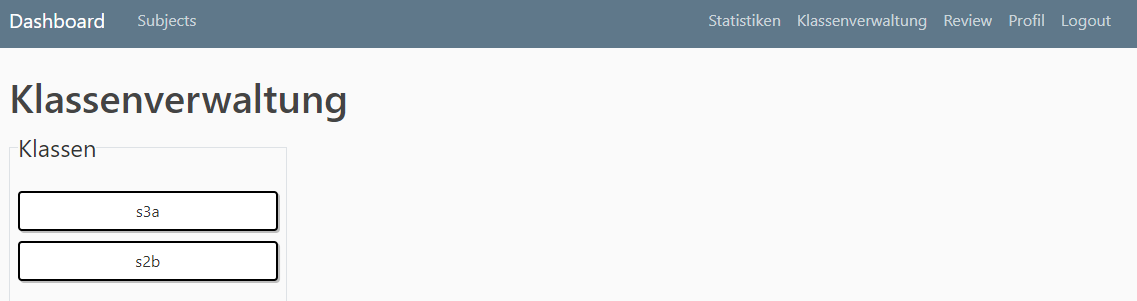
\includegraphics[width=\textwidth, height=\textheight, keepaspectratio]{images/Webseite/Klassenverwaltung_Desktop.png}
		\caption{Anpassung Klassenverwaltung}
	\end{figure}
\end{minipage}	

Nachdem eine Klasse gewählt wurde, werden die klassenspezifischen Informationen geladen und ebenfalls dargestellt. \\

\begin{minipage}{\textwidth}
	\begin{figure}[H]
		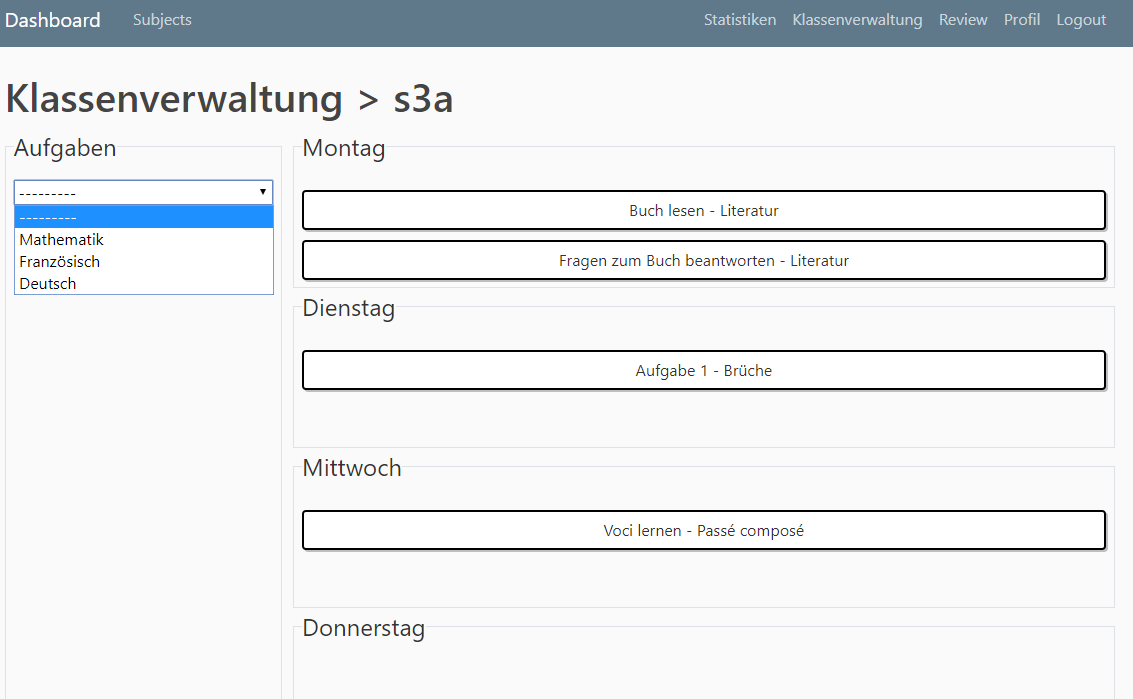
\includegraphics[width=\textwidth, height=\textheight, keepaspectratio]{images/Webseite/Klassenverwaltung_Klasse_Desktop.png}
		\caption{Informationen einer Klasse}
	\end{figure}
\end{minipage}

	\item Die Funktion um eigene Aufgaben mit anderen Lehrpersonen zu teilen wurde entfernt. Standardmässig sind nun alle erstellen Aufgaben für alle Lehrpersonen ersichtlich.
\end{itemize}




%\subsubsection{Funktionale Tests}
%Mit den geschriebenen Tests wurde eine Testcoverage von 97\% erreicht. Bei so hohen Zahlen muss man vorsichtig sein. Nur weil die Testcoverage so hoch ist, heisst es noch lange nicht, dass die Software keine Fehler aufweisst \footcite{test_coverage}. Nur weil eine Zeile Code bei einem Test durchlaufen wird, bedeutet das nicht, dass die Zeile auch getestet wurde. Grundsätzlich gibt es zwei grosse Fehler, die man beim Testen machen kann. Der erste Fehler ist es eine Testcoverage von 100\% anzustreben und sich einZUreden, dass der Code einwandfrei getestet wird. Der zweite Fehler ist es, keinen Wert auf die Testcoverage zu legen. Erreicht man Werte im Bereich von 30\% bis 40\%, ist sofort klar, dass das Testen vernachlässigt wurde. Im allgemeinen gilt, die Qualität der Tests ist ausschlaggebend. Eine hohe Testcoverage erreicht durch sinnvolle Tests ist daher ein anzustrebendes Ziel. 

\subsubsection{Performance Testing}
Um sicherzustellen, dass nichtfunktionale Anforderungen wie die Response Time und die Scalability erfüllt werden, wurden Performance Tests durchgeführt. Dafür wurde das Tool Gatling \footcite{performance_tests} verwendet. Um so realitätsgetreu und dementsprechend auch sinnvoll wie möglich zu testen, wurden 300 Schüler, 20 Lehrer und 1 Administrator simuliert, welche die Applikation verwendeten. \\

\textbf{Auswertung:} \\
Insgesamt wurden über einen Zeitraum von 2 Minuten und 15 Sekunden 28'183 Requests abgesetzt. In der Abbildung \ref{request_per_second} ist ersichtlich, wie die Requests über den erwähnten Zeitverlauf verteilt absetzt wurden.

	\begin{figure}[H]
		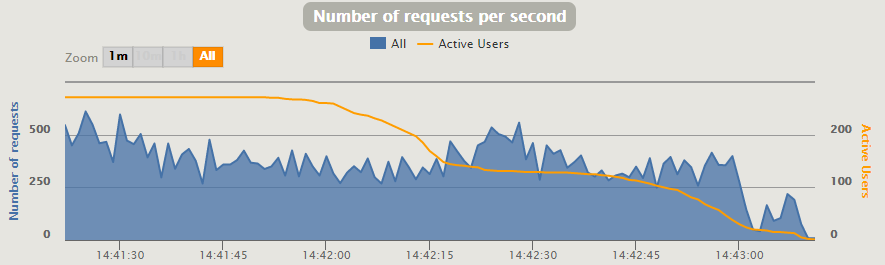
\includegraphics[width=\textwidth, height=\textheight, keepaspectratio]{images/performance_requests_per_second.png}
		\caption{Anfragen pro Sekunde}
		\label{request_per_second}
	\end{figure}

Wie in der Abbildung \ref{performance_tests} ersichtlich ist, werden die gestellten Anforderungen nicht ganz erfüllt. Die Applikation kann zwar von 300 Schülern zeitgleich verwendet werden, jedoch wurde die erwünschte Response Time von unter einer Sekunde nicht durchgehend erreicht. Bei etwa 6\% der gesendeten Anfragen, benötigte die Applikation etwas mehr als eine Sekunde. Grund dafür ist unter anderem das Laden von Bibliotheken, wie zum Beispiel 'jquery-3.1.1.min.js' und 'bootstrap.min.css', welche für die Darstellung der Seite benötigt werden. Diese Bibliotheken wurden zwar statisch in die Applikation eingebunden, was die Performance bereits stark verbesserte, jedoch noch nicht ausreicht. 

	\begin{figure}[H]
		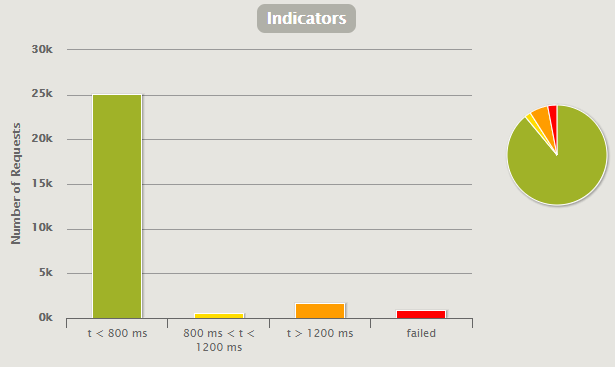
\includegraphics[width=\textwidth, height=\textheight, keepaspectratio]{images/performance_uebersicht.png}
		\caption{Performance Test Übersicht}
		\label{performance_tests}
	\end{figure}



\subsection{Code Statistiken}
Die Werte aus Tabelle \ref{cloc} wurden mit dem Tool cloc \footcite{cloc} (Count Lines of Code) generiert und zeigen, wie viele Zeilen Code im Rahmen dieser Bachelorarbeit geschrieben wurden. In die Statistik aufgenommen wurde nur selbst geschriebener Code. Alles was automatisch generiert wurde, wurde ausgeschlossen. Der Code der geschriebenen Tests ist in diesen Zahlen inbegriffen. \\


\begin{table}[h]
	\centering
	\begin{tabu} to 0.9\textwidth {l X X X}
	\toprule
		Sprache & Blank & Kommentar & Code \\ 
	\midrule
		Python & 1456 & 108 & 5501 \\
		HTML & 256 & 0 & 1087 \\
		JavaScript & 12 & 51 & 168 \\
	\bottomrule
		Summe & 1727 & 159 & 6761 \\
	\bottomrule
	\end{tabu}
	\captionof{table}{Code-Statistik}
	\label{cloc}
\end{table}
\newpage
\subsection{Ergebnisse}

\subsubsection{Resultate}
Trotz des verkürzten Zeitplans war es dennoch möglich, einen Grossteil der Funtkionen umzusetzen. Nachfolgend wird aufgelistet, welche Funktionen durch Aufgaben-Coaching ermöglicht werden. Die Liste ist auf die einzelnen User Rollen aufgeteilt.

\subsubsection*{Student}
Nachfolgend wird die Funktionalität der Schüler aufgelistet:

\begin{itemize}
	\item Einzelne Lektionen anschauen
	\item Aufgaben lösen, falls nötig auch verbessern
	\begin{itemize}
		\item Pro Frage können mehrere Hilfestellungen bereit stehen, welche dem Schüler beim Beantworten dieser Frage helfen.
	\end{itemize}
	\item Fragen im Forum stellen
\end{itemize}

\subsubsection*{Teacher}
Lehrer haben folgende Funktionalität:

\begin{itemize}
	\item Übungen erfassen und bearbeiten
	\begin{itemize}
		\item Dynamisches hinzufügen von Fragen und Hilfestellungen.
		\item Punktevergabe pro Frage.
	\end{itemize}
	\item Eigene Klassen verwalten
	\begin{itemize}
		\item Fächer einer Klasse zuweisen
		\item Aufgaben dem Wochenplan einer Klasse zuweisen
	\end{itemize}
	\item Gelöste Aufgaben korrigieren
	\begin{itemize}
		\item Filtern von allen gelösten Aufgaben seiner Schüler
		\item Pagination Ansicht der gefilterten Aufgaben
		\item Einzelne Aufgaben akzeptieren oder zurückweisen
		\item Feedback für einzelne Aufgaben erfassen
		\item Mail an Schüler mit dem Feedback schicken
	\end{itemize}
	\item Statistiken einsehen
	\begin{itemize}
		\item Von gelösten Aufgaben werden Statistiken erstellt
		\item Lehrer kann diese Statistiken einsehen und so schwächere Schüler besser unterstützen
	\end{itemize}
\end{itemize}


\subsubsection*{Admin}
Im Prinzip hat der Admin die Rechte, um alles auf der Website zu tun. Nachfolgend sind nur die Features, welche sich spezifisch an den Admin richten:

\begin{itemize}
	\item Schüler und Lehrer erfassen und bearbeiten
	\item Klassen erstellen und User diesen Klassen zuweisen
\end{itemize}


\subsubsection{Verbesserung}
Die Anwendung war viel komplexer als zu Beginn erwartet. Um im Zeitplan zu bleiben, musste bei gewissen Features  Kompromisse eingegangen werden, um dennoch im Zeitplan zu bleiben. Folgende Liste mit Features soll noch verbessert werden:

\begin{itemize}
	
\end{itemize}

\subsubsection{Weiterentwicklung}

\newpage

\section{Projektplan}
Während der Bachelorarbeit wurde der Projektplan als eigenständiges Dokument geführt. Falls Änderungen vorgekommen sind, wurde der Projektplan dementsprechend angepasst. Gegen Ende der Bachelorarbeit wurde der Projektplan in die Dokumentation eingefügt

\subsection{Inhalt}
\subsubsection*{Zweck}
Dieses Dokument beschreibt die Planung der Bachelorarbeit, in welchem eine Lernplattform für Schulen entwickelt wird.

\subsubsection*{Gültigkeitsbereich}
Dieses Dokument ist während der gesamten Laufzeit der Bachelorarbeit gültig. Die Änderungsgeschichte kann in Github nachverfolgt werden.

\subsubsection*{Referenzen}
Dieses Dokument wurde mit dem Wissen erstellt, welches in den Modulen Software Engineering 1 \& 2, der Studienarbeit sowie in gewissen Grenzen in Cloud Infrastructure und Web Engineering \& Design, vermittelt wird.



\subsection{Projektübersicht}
Bei dieser Bachelorarbeit wird eine Lernplattform erstellt, mit welchem Lehrer und Schüler zusammenarbeiten können. Auf dieser Plattform kann die Theorie der einzelnen Fächer in Form von Videos oder Theoriezusammenfassungen vermittelt werden. Zudem können Übungen erstellt und zur Verfügung gestellt werden. \\
Der Lehrer kann eigene Aufgaben erfassen, welche die Schüler lösen können. Nachdem die Aufgaben gelöst wurden, sieht der Lehrer eine Statistik, ob und wie gut die einzelnen Aufgaben gelöst wurden. Falls eine Aufgabe überdurchschnittlich schlecht gelöst wurde, kann er diese direkt im Unterricht ansprechen und allfällige Fragen klären. \\
Die Kernaufgabe dieser Bachelorarbeit ist der aufgabenspezifische Teil. Ferner kann die Plattform aber noch um zusätzliche Features wie einen Chat oder ein Forum erweitert werden.


\subsubsection*{Lieferumfang}
Folgende Dokumente werden am Ende der Bachelorarbeit abgeliefert:
\begin{itemize}
	\itemsep0em
	\item Abstract
	\item Aufgabenstellung
	\item Projektplan
	\item Projektdokumentation
	\item Installations Anleitung
	\item Bedienungs Anleitung
	\item Einverständniserklärung
	\item Erklärung zur Urheberschaft
	\item Passwörter
	\item Persönliche Berichte
	\item Protokolle
	\item Source Code	
\end{itemize}



\subsection{Organisation}
\subsubsection*{Personen und Rollen}
Nachfolgend werden alle an dieser Bachelorarbeit beteiligten Personen und ihre Rollen aufegelistet.
\subsubsection*{Luca Gubler}
Die Idee für das Thema dieser Bachelorarbeit stammt von Luca. Aus diesem Grund kümmert er sich um den groben Projektverlauf der Arbeit. Bei der Arbeit selber kümmert er sich hauptsächlich um die Infrastruktur, die Datenbank und das Backend der Applikation.

\subsubsection*{Alessandro Bonomo}
Alessandro kümmert sich hauptsächlich um das Frontend und das UI der Applikation. Er arbeitet jedoch auch am Backend mit und kümmert sich um das Testing der Applikation.

\subsubsection*{Externe Personen}
Bei dieser Bachelorarbeit übernimmt Professor Frank Koch die Rolle des Betreuers. Stephan Meier übernimmt die Rolle als externer Co-Examinators. Zusätzlich wird Professor Laurent Metzger diese Bachelorarbeit als interner Co-Examinator betreuen.

\newpage
\subsection{Management Abläufe}
\subsubsection*{Zeitbudget}
Die Bachelorarbeit begann in der Woche vom  16. September 2019 und dauert insgesamt 17 Wochen. Für das Erreichen der 12 ECTS ist geplant, dass jedes Teammitglied 360 Stunden arbeitet. Daraus resultiert eine durchschnittliche Arbeitszeit von knapp 24 Stunden pro Woche.

\begin{table}[h]
	\centering
	\begin{tabu} to 0.9\textwidth {l X}
	\toprule
	Projektstart & 13.10.2019 \\
	Projektdauer & 13 Wochen \\
	Arbeitsstunden pro Person & 23h pro Woche, Total 300h \\
	Arbeitsstunden Total & 600h \\
	Projektende & 10.01.2020 \\ 
	\bottomrule
	\end{tabu}
	\captionof{table}{Übersicht Zeitaufwand}
\end{table}


\noindent Für die Bachelorarbeit stehen total 720 Stunden zur Verfügung. Da jedoch für das erste Thema ca. 60 Arbeitsstunden pro Person aufgewendet wurden, stehen für die neue Arbeit noch total 600 Stunden zur Verfügung. Mit dem definierten Projektumfang wird diese Arbeitszeit voraussichtlich vollständig ausgenutzt. Sollte der Umfang jedoch früher als erwartet abgeschlossen werden können, kann das Projekt um weitere Funktionalitäten erweitert werden.

\subsubsection*{Projektmanagement}
Als Projektmanagement Methode wurde SCRUM+ gewählt. Bei dieser Projektmanagement Methode handelt es sich um einen Mix aus SCRUM und Unified Process. Diese Methode wird auch von Daniel Keller im Modul ''Software Engineering'' unterrichtet.

\subsubsection*{Phasen / Sprints}
Bei SCRUM+ wird das gesamte Projekt in die vier Phasen Inception, Elaboration, Construction und Transition eingeteilt. Pro Phase gibt es wiederum einzelne Sprints. Zudem wurden einzelne Meilensteine definiert, welche auf der untenstehenden Tabelle entnommen werden können.

\subsubsection*{Iterationsplanung}
Die Dauer eines Sprints wurde auf 2 Wochen festgelegt. Zu Beginn jedes Sprints setzt sich das Team zusammen um den nächsten Sprint zu planen. Dabei wird jeweils besprochen, welche Aufgaben des vergangenen Sprints nicht vollständig abgeschlossen werden konnten. Die nicht abgeschlossenen Arbeiten werden mit neu definierten Aufgaben in den neuen Sprint übernommen und jeweils zeitlich abgeschätzt und priorisiert. Da sich im Team nur 2 Mitglieder befinden, wird darauf verzichtet, die Arbeitspakete unter den Teammitgliedern  zuzuweisen. Die gesamte Planung und Verwaltung der Aufgaben wird in Jira erledigt.


\newpage
\subsubsection*{Meilensteine}
Folgende Meilensteine wurden gesetzt. Da der Projektumfang aber relativ gross war und durch den Wechsel der Projektarbeit weniger Zeit zur Verfügung stand, konnten nicht alle Meilensteine eingehalten werden. \\
Der Meilenstein ''Feature Freeze'' musste um 2 Wochen nach hinten verschoben werden. Die Zeit reichte schlicht und einfach nicht aus, um alle geforderten Funktionalitäten in der vorgenommenen Zeit umzusetzen. 

%TODO cell spacing
\begin{table}[h]
	\centering
	\begin{tabu} to 0.9\textwidth {l l X}
	\toprule
	SW & Meilenstein & Beschreibung \\ 
	\midrule
	4 & M0: Kickoff & Start des Projektes \\ 
	5 & M1: Abschluss Projektplan & Projektplan erstellt und mit Betreuer besprochen \\
	7 & M2: End of Elaboration & Use Cases und funktionale sowie nicht funktionale Anforderungen sind erfasst. Mockups Domainanalyse und Konzept für die Architektur sind erstellt. \\
	12 & M3: Feature Freeze & Entwicklung der Features ist abgeschlossen, damit man sich auf Bugfixes und Code Qualität konzentrieren kann.\\
	15 & M4: Code Freeze & Entwicklung an der Applikation ist abgeschlossen. End of Construction.\\
	17 & M5: Projektende & Abgabe der Bachelorarbeit \\ 
	\bottomrule
	\end{tabu}
	\captionof{table}{Übersicht Meilensteine}
\end{table}

\subsubsection*{Termine}
Folgende Termine sind von der \gls{hsr} oder dem Betreuer vorgegeben und müssen eingehalten werden.

%\begin{table}[h]
%	\centering
%	\begin{tabu} to 0.9\textwidth {l l X}
%	\toprule
%	Datum & Beschreibung \\ 
%	\midrule
%	6.1.1010 & Erfassung des Abstracts im Online-Tool https://abstract.hsr.ch/ Die
%Studierenden geben den Abstract für die Diplomarbeitsbroschüre zur
%Kontrolle an ihren Betreuer/Examinator frei.
%Vorlagen sowie eine ausführliche Anleitung betreffend Dokumentation
%stehen auf dem Skripteserver zur Verfügung.
%Der Betreuer/Examinator gibt das Dokument mit dem korrekten und
%vollständigen Abstract der Broschüre zur Weiterverarbeitung an das
%Studiengangsekretariat frei. \\
%	10.1.2020 & Abgabe des Berichts an den Betreuer und Hochladen aller Dokumente auf archiv-i.hsr bis 17 Uhr \\
%	10.2.2020 & Präsentation der Bachelorarbeit und mündliche Prüfung.
%	\bottomrule
%	\end{tabu}
%	\captionof{table}{Übersicht Termine}
%\end{table}

\subsection{Projektverwaltung}
%TODO JIRA workflow beschreiben
Als Projektverwaltungstool wird Jira verwendet. Man hat sich für dieses Tool entschieden, da es die gewünschte Funktionalität mit sich bringt. Um den Stand der einzelnen Arbeitspakete möglichst genau darzustellen, wurde ein Workflow definiert, welcher jedes Arbeitspaket durchlaufen muss.
%TODO BILD Workflow einfügen
%TODO ich wür review als workflow schritt use neh. wenn du arbeitspaket erfassisch, denn mussi das ned nomal aluege. review isch guet für code. wenn du doku korrigiersch, wottis ned nomal müsse aluege.
Wie im Bild ersichtlich ist, muss jedes Arbeitspaket folgende Status durchlaufen: Open, In Progress, Review und Done. Ein Arbeitspaket muss jeden Schritt im Workflow durchlaufen, ausser Review. Dieser Schritt ist optional und muss nicht bei jedem Arbeitspaket durchgeführt werden.

\subsubsection*{Zeiterfassung}
Die Zeiterfassung wird mit Jira verwaltet. Beim Einfügen von Arbeitspaketen in den Sprint wird die Zeit geschätzt, welche für das Arbeitspaket aufgewendet werden muss. Jede Person, welche an diesem Arbeitspaket gearbeitet hat, kann Zeit auf dieses Arbeitspaket buchen. Am Schluss kann so eine Zeitauswertung über die einzelnen Sprints oder das gesamte Projekt gemacht werden.

\subsubsection*{Meetings}
Die Teammitglieder arbeiten an mindestens zwei Tagen pro Woche zusammen im Bachelorarbeitszimmer. So können Fragen schnell geklärt werden und es kann sich gegenseitig geholfen werden. Im Normalfall findet jeden Donnerstag ein Meeting mit dem Betreuer Frank Koch statt, bei dem der aktuelle Stand vorgestellt, Probleme besprochen und das weitere Vorgehen geplant wird. Da der Betreuer jedoch immer wieder unterwegs war, wurde oft eine Telefonkonferenz gemacht.

\subsection{Risikomanagement}
\subsubsection*{Risiken}
Folgende Risiken sind beim Beginn der Bachelorarbeit erkannt worden:

\renewcommand{\arraystretch}{1.2}
\begin{table}[h]
	\centering
	\begin{tabu} to 0.9\textwidth {l p{0.35\textwidth} X X p{0.15\textwidth}}
	\toprule
	Nr & Beschreibung & Schaden total [h] & Eintritts-wahrsch. & Gwichteter Schaden [h]\\ 
	\midrule
	R1 & Unterschätzen des Aufwandes & 60 & 20 \% & 12 \\
	R2 & Fehldendes KnowHow von \newline Python oder Frameworks & 60 & 20 \% & 12 \\
	R3 & Konflikte im Team & 8 & 5 \% & 0.4 \\
	R4 & Schlechtes UI Design & 32 & 25 \% & 8 \\
	R5 & Technische \newline Fehlkonfigurationen & 60 & 20 \% & 12 \\
	R6 & Probleme beim Deployment & 24 & 25 \% & 6 \\ 
	R7 & Probleme mit der Architektur & 32 & 25 \% & 8 \\
	\bottomrule
	\end{tabu}
	\captionof{table}{Risikoübersicht}
\end{table}

\medskip \noindent
Daraus resultiert folgender Risikograph: 
\begin{figure}[H]
	\includegraphics[width=\textwidth,height=\textheight,keepaspectratio]{images/risikoanalyse.png}
	\caption{Risikograph}
\end{figure}

\noindent In der Inception Phase wurde ein total gewichteter Schaden von 70.7 Arbeitsstunden geschätzt. Durch gezielte Massnahmen konnte dieser Schaden auf 56.2 Arbeitsstunden vermindert werden. \\
Aufgrund dieser Annahme und weil der Zeitraum durch die Verzögerungen zu Beginn der Arbeit recht knapp bemessen ist, wurde zum Schluss der Bachelorarbeit eine Woche Bufferzeit einberechnet. 

\subsubsection*{Massnahmen}
Risiken lassen sich in einem grösseren Projekt leider nicht ganz vermeiden. Für die erfassten Risiken wurden Massnahmen definiert, um das Risiko weitgehen zu minimieren. In der nachfolgenden Tabelle sind diese Massnahmen aufgelistet.

\renewcommand{\arraystretch}{1.2}
\begin{table}[H]
	\centering
	\begin{tabu} to 0.9\textwidth {l X X}
	\toprule
	Nr & Vorbeugung & Verhalten beim Eintreten \\ 
	\midrule
	R1 & Reserven einplanen und Abgrenzung des Scopes & Reserven nutzen und notfalls den Scope anpassen \\
	R2 & In der Elaboration Phase Zeit einplanen, um sich in die einzelnen Phasen einarbeiten zu können & Fehlendes KnowHow aufbauen, gegebenenfalls mit Unterstützung des anderen Teammitgliedes \\
	R3 & Zusammenarbeit im Team und gegenseitige Absprache & Notfalls Gespräch mit dem Betreuer \\
	R4 & Mockups erstellen und Usability Tests mit externen Personen durchführen & User Interface anpassen \\
	R5 & KnowHow in der Elaboration Phase aufbauen und für den Notfall Backups erstellen & Restore der Backups und redeployment des Systems \\
	R6 & Vorläufig testen, wie eine Applikation deployed wird & Genauere Recherche, wie das Deployment funktioniert \\
	R7 & Architektur so planen, dass sie einfach erweitert und angepasst werden kann & Architektur anpassen \\
	\bottomrule
	\end{tabu}
	\captionof{table}{Massnahmen}
\end{table}

\subsubsection*{Auswertung}
Während der gesamten Projektdauer sind eigentlich nur zwei der oben genannten Risiken aufgetreten. Ein grosses Problem war das fehlende KnowHow des Django Frameworks. Besonders zu Beginn der Projektarbeit gab es oft Fragen und Unklarheiten, welche zuerst geklärt werden mussten. \\
Dies führte unweigerlich zum zweiten Risiko, nämlich des sehr knapp bemessenen Zeitraums. Durch den Wechsel des Bachelorarbeits Thema standen 4 Wochen weniger Zeit zur Verfügung. Gegen Ende der Arbeit wurde immer deutlicher, dass nicht der gesamte Scope abgedeckt werden kann. Dies wurde jedoch mit dem Betreuer abgesprochen und der Scope wurde dementsprechend angepasst. Auf Features wie das aufgaben-spezifische Forum wurden somit verzichtet.

\subsection{Qualitätsmanagement}

\subsubsection*{Dokumentation}
Die Dokumentation der Bachelorarbeit wird mit \LaTeX und in einem eigens dafür eingerichteten Git Repository gemacht. Somit ist es möglich, jede Änderung an der Dokumentation zu verfolgen. Wird ein Kapitel geschrieben, wird es vom anderen Teammitglied gegen gelesen und falls nötig angepasst. Somit stammt die Dokumentation von beiden Teammitgliedern und repräsentiert nicht die Meinung einer einzelnen Person. 

%\subsubsection*{Projektmanagement}
%Als Projektmanagement Tool wird Jira verwendet. Dieses Tool bietet zwar sehr viele Features, die für die Bachelorarbeit gar nicht benötigt werden. Man hat sich aber auf Jira festgelegt, weil bereits Erfahrungen, unter anderem während der Studienarbeit, gesammelt wurden. \\
%Alle Arbeitspakete werden in Jira aufgenommen und mit einer geschätzten Arbeiszeit versehen. Zudem muss jedes Arbeispaket einen zuvor bestimmten Workflow durchlaufen. Wird ein Arbeispaket dem Sprint zugewiesen, hat es zuerst den Status ''Open''. Wird das Arbeispaket bearbeitet, bekommt es den Status ''In progress''. Je nach Typ von Arbeitspaket kommt es anschliessend zu ''Review'' oder ''Finished''. Arbeispakete können nicht direkt von ''Open'' zu ''Finished'' gehen. Der Schritt ''Review'' ist jedoch optional und wird nur falls nötig durchlaufen.

\subsubsection*{Entwicklung}
Der gesamte Source Code befindet sich auf Github. Der master Branch wird als protected Branch eingerichtet. Ein Branch kann also nicht direkt in den Master Branch gemerged werden, sonder muss mittels eines Pull Requests gemerged werden. Dies hat den Vorteil, dass sämtlicher Code das Vier-Augen Prinzip durchlaufen hat. \\ 
Zudem wird Travis CI verwendet, welches nach jedem Push die selbst geschriebenen Tests durchführt. Somit kann man sich auch sicher sein, dass sämtlicher Code auch wirklich alle Tests besteht.

\subsubsection*{Code Reviews}
Bei jedem Pull Request wird auch gleich ein Code Review durchgeführt. Dies hat den Vorteil, dass der Code, welcher in den Master Branch gemerged wird, auch den Anforderungen beider Teammitglieder entspricht.

\subsubsection*{Tools und Infrastruktur}
Für die Infrastruktur werden lediglich 2 Notebooks und ein Server benötigt. Die Notebooks stammen von den Diplomanden und der Server wird durch die \gls{hsr} zur Verfügung gestellt. \\
Als IDE wurde entschieden, sich auf PyCharm von JetBrains zu beschränken. Dies hat den Vorteil, dass man sich beim Pair-Programming schnell zurecht findet. \\
Als Projektmanagement Tool wird Jira eingesetzt. \\
Die Dokumentation und der Projektplan werden mit \LaTeX erstellt. Kleinere Dokumente oder das Sitzungsprotokoll werden mit Word erfasst. 

\newpage
\section{Software Dokumentation}
Dokumentation als PDF einfügen
\section{Dankausgang}
Den Leuten danken, die geholfen haben
\section{Fazit}
Der Anfang der Bachelorarbeit war ein wenig chaotisch. Während 4 Wochen arbeiteten wir an einem anderen Thema. Aufgrund mehrerer Vorkommnisse waren wir aber gezwungen, das Thema der Arbeit zu wechseln. Dadurch ging jedoch knapp 20\% der Zeit verlorem. Da das neue Thema aber einen relativ grossen Umfang hatte, war es während der Arbeit nicht immer einfach. Viele der eingesetzten Technologien waren neu und man musste sich zuerst einarbeiten. Dies führte schlussendlich zu einem relativ strikt getakteten Zeitplan. \\

Nach Abschluss der Arbeit können wir aber sagen, dass wir stolz auf die erreichten Ergebnisse sind. Besonders toll war, dass wir unsere eigene Idee als Bachelorarbeit umsetzen konnten. Wir waren auch beim Erstellen der Aufgabenstellung involviert und konnten unsere eigenen Ideen einbringen. Zudem ist es toll, dass wir eine Arbeit erstellen konnten, welche nicht einfach zum erhalten des Bachelor Diploms dient, sondern nach Abschluss des Studiums weiter entwickelt werden soll.



%%%%%%%%%%%%%%%%%%%%%%%%%%%%%%
% List of figures & glossary %
%%%%%%%%%%%%%%%%%%%%%%%%%%%%%%
\listoffigures
\listoftables
\printnoidxglossaries

%%%%%%%%%%%%%%%%
% Bibliography %
%%%%%%%%%%%%%%%%
%\bibliographystyle{abbrv}
%\bibliography{index/bibliography}
\printbibliography

%%%%%%%%%%%%%%%%%%%%
% Attached sources %
%%%%%%%%%%%%%%%%%%%%
\input{attachments/attachments}


\end{document}